% !TeX TXS-program:compile = txs:///pdflatex/[--shell-escape]
%
% acm templates v1.57 (sigconf template)
%
%\documentclass[sigconf, screen, review, anonymous, natbib=false]{acmart}
\documentclass[sigconf, screen, natbib=false, dvipsnames, table]{acmart}
\settopmatter{printacmref=true}
% mandatory for CCS'19
\usepackage{balance}
\usepackage{mathtools}
% for creating a balanced last page (usually last page with references)

% % defining the \BibTeX command - from Oren Patashnik's original BibTeX documentation.
% \def\BibTeX{{\rm B\kern-.05em{\sc i\kern-.025em b}\kern-.08emT\kern-.1667em\lower.7ex\hbox{E}\kern-.125emX}}

% Rights management information.
% This information is sent to you when you complete the rights form.
% These commands have SAMPLE values in them; it is your responsibility as an author to replace
% the commands and values with those provided to you when you complete the rights form.
%
% These commands are for a PROCEEDINGS abstract or paper.

\copyrightyear{2019}
\acmYear{2019}
\setcopyright{acmcopyright}
\acmConference[CCS '19]{2019 ACM SIGSAC Conference on Computer and Communications Security}{November 11--15, 2019}{London, United Kingdom}
\acmBooktitle{2019 ACM SIGSAC Conference on Computer and Communications Security (CCS '19), November 11--15, 2019, London, United Kingdom}
\acmPrice{15.00}
\acmDOI{10.1145/3319535.3339818}
\acmISBN{978-1-4503-6747-9/19/11}

%
% These commands are for a JOURNAL article.
%\setcopyright{acmcopyright}
%\acmJournal{TOG}
%\acmYear{2018}\acmVolume{37}\acmNumber{4}\acmArticle{111}\acmMonth{8}
%\acmDOI{10.1145/1122445.1122456}

%
% Submission ID.
% Use this when submitting an article to a sponsored event. You'll receive a unique submission ID from the organizers
% of the event, and this ID should be used as the parameter to this command.
%\acmSubmissionID{123-A56-BU3}

%
% The majority of ACM publications use numbered citations and references. If you are preparing content for an event
% sponsored by ACM SIGGRAPH, you must use the "author year" style of citations and references. Uncommenting
% the next command will enable that style.
%\citestyle{acmauthoryear}


 \makeatletter
 % \renewcommand{\section}{\abovedisplayskip 10\p@ \@plus3\p@ \@minus1\p@%
 %                       \belowdisplayskip 5\p@ \@plus3\p@ \@minus1\p@%
 %                       \abovedisplayshortskip 0pt \@plus2\p@%
 %                       \belowdisplayshortskip 0pt \@plus2\p@ \@minus0\p@%
 %                       \@startsection{section}{1}{\z@}%
 %                        {-17\p@ \@plus -4\p@ \@minus -4\p@}%
 %                        {6\p@ \@plus 4\p@ \@minus 4\p@}%
 %                        {\normalfont\large\bfseries\boldmath
 %                         \rightskip=\z@ \@plus 8em\pretolerance=10000 }}
 \renewcommand{\subsection}{\@startsection{subsection}{2}{\z@}%
                        {-8\p@ \@plus -4\p@ \@minus -4\p@}%
                        {5\p@ \@plus 2\p@ \@minus 2\p@}%
                        {\normalfont\Large\bfseries\boldmath
                         \rightskip=\z@ \@plus 3em\pretolerance=10000 }}
  \renewcommand{\subsubsection}{\@startsection{subsubsection}{3}{\z@}%
                        {-6\p@ \@plus -4\p@ \@minus -4\p@}%
                        {1\p@ \@plus 1\p@ \@minus 0\p@}%
                        {\normalfont\normalsize\bfseries\boldmath}}
% \renewcommand{\paragraph}{\@startsection{paragraph}{4}{\z@}%
%                       {-8\p@ \@plus -4\p@ \@minus -4\p@}%
%                       {-2\p@ \@plus -0.22em \@minus -0.1em}%
%                       {\normalfont\normalsize\bfseries}}
 \makeatother



% *** GRAPHICS RELATED PACKAGES ***
\usepackage{graphicx}
\usepackage{comment}
\usepackage{amsmath,amssymb,amsfonts}
\usepackage{listings}
% declare the path(s) where your graphic files are
\graphicspath{{../figures/}}
% and their extensions so you won't have to specify these with
% every instance of \includegraphics
\DeclareGraphicsExtensions{.pdf,.jpeg,.png}

% Minted is used for source code highlighting
%\usepackage[outputdir=/Volumes/ramdisk/]{minted}
% \usepackage{minted}
% *** MATH PACKAGES ***
\usepackage{amsmath}



% *** SPECIALIZED LIST PACKAGES ***
%\usepackage{algorithm2e}
\usepackage{algorithmic}



% *** ALIGNMENT PACKAGES ***
\usepackage{array}

\usepackage{url}

\usepackage[utf8]{inputenc}
\usepackage[american]{babel}
\usepackage[backend=biber,style=ACM-Reference-Format]{biblatex}
\addbibresource{./library.bib}
\addbibresource{./cryptobib/abbrev2.bib}
\addbibresource{./cryptobib/crypto_crossref.bib}

% Used for Theorems and Definitions
\usepackage{amsthm}
\newtheorem{definition}{Definition}
\newtheorem{theorem}{Theorem}
\newtheorem{lemma}{Lemma}
\theoremstyle{definition}
\newtheorem{remark}{Remark}
\newtheorem{assumption}{Assumption}

\usepackage{xcolor}
\usepackage{xspace}
\usepackage{xstring} % required by IfEqCase

\usepackage{booktabs} % better tables
\usepackage{algorithm}
\usepackage{algorithmic}

% for references, use it like this: \cref{some_label}
% it will automatically put Appendix, Figure, Section, etc before the reference
\usepackage[capitalise]{cleveref}

% ishaq: adding our macros

% the following commands require xcolor and xpace packages
\newcommand{\vassilis}[1]{{\color{blue} {\sc Vassilis:} \it #1}\xspace}
\newcommand{\vvassilis}[1]{{\color{blue} \footnote{\vassilis{#1}}}}
%\renewcommand{\vvassilis}[1]{\vassilis{#1}}

\newcommand{\ana}[1]{{\color{red} {\sc Ana:} \it #1}\xspace}
\newcommand{\aana}[1]{{\color{red} \footnote{\ana{#1}}}}
\newcommand{\ishaq}[1]{{\color{teal} {\sc Ishaq:} \it #1}\xspace}
\newcommand{\iishaq}[1]{{\color{teal} \footnote{\ishaq{#1}}}}
\newcommand{\ben}[1]{{\color{orange} {\sc Ben:} \it #1}\xspace}
\newcommand{\bben}[1]{{\color{orange} \footnote{\ben{#1}}}}
\newcommand{\benjamin}[1]{{\color{green} {\sc Benjamin:} \it #1}\xspace}

\newcommand{\revised}[1]{#1}
\newcommand{\brevised}[1]{{\color{blue} #1}}

\newcommand{\rrefer}[2]{%
    \IfEqCase{#1}{%
        {proceedings}{\revised{See full version for details.}}%
        {full}{\revised{See appendix~\ref{#2} for details.}}%
        % you can add more cases here as desired
    }[\PackageError{rrefer}{Undefined option for arg1 #1}]%
}
\newcommand{\refer}[1]{\rreferx{proceedings}{#1}}

\newcommand{\rrefr}[3]{%
    \IfEqCase{#1}{%
        {proceedings}{\revised{#2}}%
        {full}{\revised{#3}}%
        % you can add more cases here as desired
    }[\PackageError{rrefr}{Undefined option for arg1 #1}]%
}
\newcommand{\refr}[2]{\rrefr{proceedings}{#1}{#2}}

\newcommand{\para}[1]{\ensuremath{{\textsf{Parallel} (#1)}\xspace}}

% macros for notation
%\newcommand{\G}{\ensuremath{\mathcal{G}}\xspace}
\newcommand{\PA}{\ensuremath{\mathsf{PA}}\xspace}
%\newcommand{\C}{\ensuremath{\mathcal{C}}\xspace}
\newcommand{\mG}{\ensuremath{\bar{\mathcal{G}}}\xspace}
\newcommand{\scheduler}{\ensuremath{\tt S}\xspace}
\newcommand{\PPI}{\ensuremath{\Pi}\xspace}
\newcommand{\pcost}{\ensuremath{c}\xspace}
\newcommand{\fcost}{\ensuremath{\text{Cost}}\xspace}
\newcommand{\scost}{\ensuremath{c}\xspace}
\newcommand{\BB}{\ensuremath{B}\xspace}
\newcommand{\bb}{\ensuremath{B}\xspace}
\newcommand{\sss}{\ensuremath{\sigma}\xspace}
\newcommand{\SSS}{\ensuremath{\Sigma}\xspace}
\newcommand{\pibgw}{\ensuremath{\pi^{A}}\xspace}
\newcommand{\piyao}{\ensuremath{\pi^{Y}}\xspace}


% Ana's macros
\newcommand{\f}{{\sf f}\xspace}
\newcommand{\m}{{\sf m}\xspace}
\newcommand{\n}{{\sf n}\xspace}
\newcommand{\p}{{\sf p}\xspace}
\newcommand{\w}{{\sf {w}}\xspace}
\newcommand{\x}{{\sf {x}}\xspace}
\newcommand{\y}{{\sf y}\xspace}
\newcommand{\z}{{\sf z}\xspace}
\renewcommand{\varv}{{\sf v}\xspace}
\newcommand{\D}{{\sf D}\xspace}
\newcommand{\new}{{\sf new}\xspace}
\newcommand{\this}{{\sf this}\xspace}
\newcommand{\unit}{{\sf unit}\xspace}
\newcommand{\ret}{{\sf ret}\xspace}
% macros for reference (ana)
\newcommand\secref[1]{\S\ref{#1}}
\newcommand\figref[1]{Fig.~\ref{#1}}


\newcommand{\op}{{\sf aop}\xspace}
\newcommand{\cop}{{\sf bop}\xspace}
\newcommand{\ol}[1]{\overline{#1}}
\newcommand{\code}[1]{{\sf #1}\xspace}
\newcommand{\squad}{\;\;\;}
\newcommand{\trule}[1]{\textsc{\scriptsize ({#1})}}

\lstset{% general command to set parameter(s)
    basicstyle=\linespread{0.8}\sffamily\small,
    numbers=left,
    xleftmargin=16pt,
    escapechar=@,
    tabsize=2,
    columns=fullflexible
}

  \newcommand{\vnote}[1]{\stepcounter{notecount}\todo[inline,bordercolor=borderamber,linecolor=borderamber,color=lightamber]{\footnotesize{\sc \bf Vassilis:} #1}{}}

\newcommand{\A}{\ensuremath{\pi^\mathtt{A}}\xspace}
\newcommand{\B}{\ensuremath{\pi^\mathtt{B}}\xspace}
\newcommand{\Y}{\ensuremath{\pi^\mathtt{Y}}\xspace}
\newcommand{\tA}{\ensuremath{\mathtt{A}}\xspace}
\newcommand{\tB}{\ensuremath{\mathtt{B}}\xspace}
\newcommand{\tY}{\ensuremath{\mathtt{Y}}\xspace}
\newcommand{\sh}[1]{\ensuremath{\langle #1\rangle}\xspace}
\newcommand{\sconv}[1]{\ensuremath{\tt #1}\xspace}

\newcommand{\impmpc}{\text{IMP-MPC}\xspace}
\newcommand{\source}{\ensuremath{S}\xspace}
\newcommand{\cmpc}[1]{\ensuremath{C_{\text{\tiny MPC}} (#1)}\xspace}
\newcommand{\cssa}[1]{\ensuremath{C_{\text{\tiny SSA}} (#1)}\xspace}
\newcommand{\linear}[1]{\ensuremath{{\textsf{Linear} (#1)}\xspace}}
\newcommand{\sst}{\ensuremath{\texttt{st}}\xspace}


\newlength{\saveparindent}
\setlength{\saveparindent}{\parindent}
\newlength{\saveparskip}
\setlength{\saveparskip}{\parskip}


\newcounter{ctr}
\newcounter{savectr}
\newcounter{ectr}

\newenvironment{tiret}{%
\begin{list}{\hspace{1pt}\rule[0.5ex]{6pt}{1pt}\hfill}{\labelwidth=15pt%
\labelsep=3pt \leftmargin=18pt \topsep=1pt%
\setlength{\listparindent}{\saveparindent}%
\setlength{\parsep}{\saveparskip}%
\setlength{\itemsep}{1pt}}}{\end{list}}

\newenvironment{eenum}{%
\begin{list}{{\rm (\arabic{ctr}.\arabic{ectr})}\hfill}{\usecounter{ectr}%
\labelwidth=28pt\labelsep=6pt \leftmargin=34pt \topsep=0pt%
\setlength{\listparindent}{\saveparindent}%
\setlength{\parsep}{\saveparskip}%
\setlength{\itemsep}{2pt} }}{\end{list}}

\newenvironment{newenum}{%
\begin{list}{{\rm \arabic{ctr}.}\hfill}{\usecounter{ctr}\labelwidth=5pt%
\labelsep=6pt \leftmargin=11pt \topsep=.5pt%
\setlength{\listparindent}{\saveparindent}%
\setlength{\parsep}{\saveparskip}%
\setlength{\itemsep}{5pt} }}{\end{list}}

\newenvironment{neweenum}{%
\begin{list}{{\rm \arabic{ctr}.\arabic{ectr}}\hfill}{\usecounter{ectr}%
\labelwidth=28pt\labelsep=4pt \leftmargin=34pt \topsep=0pt%
\setlength{\listparindent}{\saveparindent}%
\setlength{\parsep}{\saveparskip}%
\setlength{\itemsep}{2pt} }}{\end{list}}

\newenvironment{parenum}{%
\begin{list}{{\rm (\arabic{ctr})}\hfill}{\usecounter{ctr}\labelwidth=17pt%
\labelsep=6pt \leftmargin=23pt \topsep=.5pt%
\setlength{\listparindent}{\saveparindent}%
\setlength{\parsep}{\saveparskip}%
\setlength{\itemsep}{5pt} }}{\end{list}}


%PYTHON and CODE MACROS

\definecolor{keyword}{HTML}{37AC4A}
\definecolor{operator}{HTML}{A51DFF}
\definecolor{string}{HTML}{C03333}
\definecolor{background}{HTML}{F7F7F7}


\lstdefinelanguage{python}{
  xleftmargin=4mm,
  numbers=left,
  numbersep=2mm,
  numberstyle=\tiny\color{gray},
  basicstyle=\fontsize{10}{11}\ttfamily,
  columns=flexible,
  basewidth=0.45em,
  morestring=[b]',
  morestring=[b]",
  morestring=[b]""",
  stringstyle=\textcolor{string},
  showstringspaces=false,
  morecomment=[l]\#,
  morekeywords={and,as,assert,break,class,continue,def,del,elif,else,except,False,finally,for,from,global,if,import,in,is,lambda,None,nonlocal,not,or,pass,raise,return,True,try,while,with,yield,delete,self},
  keywordstyle=\color{keyword}\bf\ttfamily,
  otherkeywords={|,>>,\&,=,<,>,**},
  morekeywords=[2]{|,>>,\&,=,<,>,**},
  keywordstyle=[2]\color{operator}\bf\ttfamily,
}

\newcommand{\python}[1]{\lstinline[language=python]{#1}}

\lstset{basicstyle=\ttfamily,
  showstringspaces=false,
  commentstyle=\color{darkgray},
  keywordstyle=\color{blue}
}

\lstnewenvironment{pythonn}
{\lstset{language=python,
  basicstyle=\small\sffamily,
  tabsize=2,
  xleftmargin=10pt,
  numbers=left,
  numberstyle=\tiny,
  numbersep=2mm,
  columns=fullflexible,
  captionpos=b,
  escapechar=\%}}  {}

\lstdefinelanguage{cpp}{
  xleftmargin=4mm,
  numbers=left,
  numbersep=2mm,
  numberstyle=\tiny\color{gray},
  basicstyle=\fontsize{10}{11}\ttfamily,
  columns=flexible,
  basewidth=0.45em,
  morestring=[b]',
  morestring=[b]",
  morestring=[b]""",
  stringstyle=\textcolor{string},
  showstringspaces=false,
  morecomment=[l]\\\\,
  morekeywords={for,if,true,false},
  keywordstyle=\color{keyword}\bf\ttfamily,
  otherkeywords={|,>>,\&,=,<,>,*},
  morekeywords=[2]{|,>>,\&,=,<,>,*},
  keywordstyle=[2]\color{operator}\bf\ttfamily,
}

\newcommand{\cpp}[1]{\lstinline[language=cpp]{#1}}

\lstset{basicstyle=\ttfamily,
  showstringspaces=false,
  commentstyle=\color{darkgray},
  keywordstyle=\color{blue}
}

\lstnewenvironment{cppp}
{\lstset{language=C++, %cppp,
  basicstyle=\small\sffamily,
  tabsize=2,
  xleftmargin=10pt,
  numbers=left,
  numberstyle=\tiny,
  numbersep=2mm,
  columns=fullflexible,
  captionpos=b,
  escapechar=\%}}  {}

%\newcommand{\trule}[1]{\textsc{\scriptsize ({#1})}}

\newenvironment{semantics}{
  \begin{displaymath}}{
  \end{displaymath}
}
\newcommand{\ntyperule}[3]{
  \begin{array}{c}
    \textsc{\scriptsize ({#1})} \\
    #2 \\[1mm]
    \hline
    \raisebox{0pt}[12pt][0pt]{\ensuremath{#3}}
  \end{array}}



\sloppy
\begin{document}
\fancyhead{}
% do not delete this code.

%
% paper title
% Titles are generally capitalized except for words such as a, an, and, as,
% at, but, by, for, in, nor, of, on, or, the, to and up, which are usually
% not capitalized unless they are the first or last word of the title.
% Linebreaks \\ can be used within to get better formatting as desired.
% Do not put math or special symbols in the title.
\title[Scheduling and Vectorization for MPC]{Scheduling and Vectorization for MPC}

%
% The "author" command and its associated commands are used to define the authors and their affiliations.
% Of note is the shared affiliation of the first two authors, and the "authornote" and "authornotemark" commands
% used to denote shared contribution to the research.

\author{Benjamin Levy}
\email{levyb3@rpi.edu}
\affiliation{%
    \institution{Rensselaer Polytechnic Institute}
    %\streetaddress{1 Th{\o}rv{\"a}ld Circle}
    \city{Troy}
    \state{New York}
    %\country{Iceland}
}

\author{Benjamin Sherman}
\email{shermb@rpi.edu}
\affiliation{%
    \institution{Rensselaer Polytechnic Institute}
    %\streetaddress{1 Th{\o}rv{\"a}ld Circle}
    \city{Troy}
    \state{New York}
    %\country{Iceland}
}


\author{Lindsey Kennard}
\email{kennal@rpi.edu}
\affiliation{%
    \institution{Rensselaer Polytechnic Institute}
    %\streetaddress{1 Th{\o}rv{\"a}ld Circle}
    \city{Troy}
    \state{New York}
    %\country{Iceland}
}

\author{Ana L. Milanova}
\email{milanova@cs.rpi.edu}
\affiliation{%
    \institution{Rensselaer Polytechnic Institute}
    %\streetaddress{1 Th{\o}rv{\"a}ld Circle}
    \city{Troy}
    \state{New York}
    %\country{Iceland}
}

\author{Muhammad Ishaq}
\authornote{This work was done in part while the author was at RPI.}
\email{m.ishaq@ed.ac.uk}
%\orcid{1234-5678-9012}
%\author{G.K.M. Tobin}
%\authornotemark[1]
%\email{webmaster@marysville-ohio.com}
\affiliation{%
    \institution{University of Edinburgh}
    %\streetaddress{P.O. Box 1212}
    \city{Edinburgh}
    \state{Scotland}
%    \postcode{43017-6221}
}

\author{Vassilis Zikas}
\authornote{This work was done in part while the author was visiting UCLA and supported in part by DARPA and SPAWAR under contract N66001-15-C-4065 and by a SICSA Cyber Nexus Research Exchanges grant.}
\email{vzikas@inf.ed.ac.uk}
%\orcid{1234-5678-9012}
%\author{G.K.M. Tobin}
%\authornotemark[1]
%\email{webmaster@marysville-ohio.com}
\affiliation{%
    \institution{University of Edinburgh}
    %\streetaddress{P.O. Box 1212}
    \city{Edinburgh}
    \state{Scotland}
    %    \postcode{43017-6221}
}


%
% By default, the full list of authors will be used in the page headers. Often, this list is too long, and will overlap
% other information printed in the page headers. This command allows the author to define a more concise list
% of authors' names for this purpose.
%\renewcommand{\shortauthors}{Trovato and Tobin, et al.}

\renewcommand{\A}{{\sf A}}
\renewcommand{\B}{{\sf B}}
\renewcommand{\C}{{\sf C}}
\renewcommand{\D}{{\sf D}}


% As a general rule, do not put math, special symbols or citations
% in the abstract
\begin{abstract}


\end{abstract}


%
% The code below is generated by the tool at http://dl.acm.org/ccs.cfm.
% Please copy and paste the code instead of the example below.
%
\begin{CCSXML}
<ccs2012>
<concept>
<concept_id>10003752.10010124.10010138.10010143</concept_id>
<concept_desc>Theory of computation~Program analysis</concept_desc>
<concept_significance>500</concept_significance>
</concept>
<concept>
<concept_id>10003752.10003777.10003789</concept_id>
<concept_desc>Theory of computation~Cryptographic protocols</concept_desc>
<concept_significance>500</concept_significance>
</concept>
<concept>
<concept_id>10002978.10002979</concept_id>
<concept_desc>Security and privacy~Cryptography</concept_desc>
<concept_significance>300</concept_significance>
</concept>
</ccs2012>
\end{CCSXML}

\ccsdesc[500]{Theory of computation~Program analysis}
\ccsdesc[500]{Theory of computation~Cryptographic protocols}
\ccsdesc[300]{Security and privacy~Cryptography}

%
% Keywords. The author(s) should pick words that accurately describe the work being
% presented. Separate the keywords with commas.
\keywords{multiparty computation; compilers; cryptography}


\begin{comment}
%
% A "teaser" image appears between the author and affiliation information and the body
% of the document, and typically spans the page.
\begin{teaserfigure}
    \includegraphics[width=\textwidth]{sampleteaser}
    \caption{Seattle Mariners at Spring Training, 2010.}
    \Description{Enjoying the baseball game from the third-base seats. Ichiro Suzuki preparing to bat.}
    \label{fig:teaser}
\end{teaserfigure}
\end{comment}
%
% This command processes the author and affiliation and title information and builds
% the first part of the formatted document.
\maketitle


\section{Introduction}
\label{sec:introduction}

\begin{itemize}
\item We define the scheduling problem for MPC. 
We present an analytical model to reason about cost of schedules
and show that scheduling is NP-hard via a reduction to the shortest 
common supersequence problem.

\item We present a compiler that takes an IMP-like high-level 
program and produces amortized (i.e., vectorized) low-level cryptographic 
code in the MOTION framework. Central contributions are 1) a novel compiler framework, 
2) a vectorization algorithm that produces optimal schedules for a large 
number of MPC programs, and 3) reasoning over output arrays without Array SSA; we remove 
infeasible loop-carried dependences introduced by standard SSA to improve vectorization.


\item We present an implementation and evaluation in the MOTION framework. 
\ana{Fill in with final results. Mention benchmarks (standard + new ones + HyCC). }


\end{itemize}

\section{Overview}
\label{sec:overview}

\subsection{Source}

As a running example, consider Biometric matching, a standard MPC benchmark.
Array \texttt{C} is the feature vector of \texttt{D} features that we wish to match and array \texttt{S} 
is the database of \texttt{N} vectors of size \texttt{D} that we match against.
An intuitive implementation is as follows:

{\small
\begin{verbatim}
def biometric(C: shared[list[int]], D: int, 
              S: shared[list[int]], N: int) -> 
                      tuple[shared[int], shared[int]]:
    min_sum = 10000
    min_index = 0  
    for i in range(N): #loop over database
        sum = 0
        for j in range(D): #loop over features
            d = S[i * D + j] - C[j] #i.e., d = S[i,j] - C[j]
            p = d * d
            sum = sum + p
        if sum < min_sum:
            min_sum = sum
            min_index = i
    return (min_sum, min_index)
\end{verbatim}
}

Our compiler takes (essentially) standard IMP syntax.
The programmer can write intuitive iterative programs as the one above.
They annotate certain inputs and outputs as \emph{shared}.
Here the code iterates over the entries in the database and computes
the sum of squares of the differences of individual features. The program returns the 
index \texttt{i} of the vector that gives the best match plus the corresponding sum of squares.


Our compiler imposes the following restrictions. We note that in some cases, the restrictions 
can be easily lifted and we plan to do so in future iterations of our compiler. 

\begin{enumerate}
\item The program contains arbitrarily nested loops, however, loop bounds are fixed: \texttt{0 <= i < N}.
A standard restriction in MPC is that the bounds must be known at circuit-generation time.
\item Arrays are one-dimensional. N-dimensional arrays are linearized and accessed 
in row-major order and at this point the programmer is responsible for linearization
and access. 
\item Array subscrpts are plaintext values.
\item Our compiler allows for output (write) arrays, however it restricts
write access to \emph{canonical writes} along the dimensions of the array. I.e., \texttt{A[i,j] = ...}
where \texttt{i} and \texttt{j} loop over the two dimensions of \texttt{A} is allowed, 
but \texttt{A[i,j+2] = ...} is not allowed. Read access is arbitrary. 
\end{enumerate}

\subsection{MPC Source and Cost of Schedule}

The compiler generates an IR, MPC source:
{\small
\begin{verbatim}
1. min_sum!1 = 10000
2. min_index!1 = 0
3. for i in range(0, N!0):
4.    min_sum!2 = PHI(min_sum!1, min_sum!4)
5.    min_index!2 = PHI(min_index!1, min_index!4)
6.    sum!2 = 0
7.    for j in range(0, D!0):
8.      sum!3 = PHI(sum!2, sum!4)
9.      d!3 = (S!0[((i * D!0) + j)] - C!0[j]) // MPC
10.     p!3 = (d!3 * d!3) // MPC
11.     sum!4 = (sum!3 + p!3) // MPC
12.  !1!2 = (sum!3 < min_sum!2) // MPC
13.  min_sum!3 = sum!3
14.  min_index!3 = i
15.  min_sum!4 = MUX(!1!2, min_sum!3, min_sum!2) // MPC
16.  min_index!4 = MUX(!1!2, min_index!3, min_index!2) // MPC
17.!2!1 = (min_sum!2, min_index!2)   
\end{verbatim}
}

The compiler linearizes the source turning conditionals into MUX statements. The PHI nodes
are remnants of the SSA IR; the compiler generates code that picks the correct value 
when producing MOTION output; the MOTION framework in turn linearizes 
loops when it generates the circuit.

We turn to our analytical model to compute the cost of this program. Assuming fixed 
cost $\beta$ for a local MPC operation (essentially just ADD) and cost $\alpha$ for a remote
MPC operation (e.g., MUX, CMP, and remaining operations), the cost of the iterative schedule 
will be $N*D*(2*\alpha+\beta) + N*3*\alpha$. 

A key contribution is the vectorizing transformation. We can compute all $N*D$ 
subtraction operations (line 9) in a single SIMD instruction; similarly we can compute 
all multiplication operations (line 10) in a single SIMD instruction. And while we cannot
vectorize computation of the N individual sums, we can compute the N sums in parallel. 
Our compiler \emph{automatically detects these opportunities and transforms the program}. 
It is standard that MPC researchers write vectorized versions of the Biometric
program by hand; we are the first (to the best of our knowledge) to automatically 
transform an intuitive, iterative MPC program into an unintuitive vectorized one.

\subsection{Vectorized MPC Source and Cost of Schedule}

Our compiler produces the following vectorized program. (Note that this is
still higher-level IR, Vectorized MPC Source. Our compiler turns this code into MOTION variables, 
loops and SIMD primitives, which MOTION then uses to generate the circuit.)

{\small
\begin{verbatim}
min_sum!1 = 10000
min_index!1 = 0
// S!0^ is same as S!0. C!0^ replicates C!0 N-times: 
S!0^ = raise_dim(S!0, ((i * D!0) + j), (i:N!0,j:D!0))
C!0^ = raise_dim(C!0, j, (i:N!0,j:D!0))

sum!2 = [0,..,0]
// Computes all differences and all products "at once"
d!3[I,J] = SUB_SIMD(S!0^[I,J],C!0^[I,J])
p!3[I,J] = MUL_SIMD(d!3[I,J],d!3[I,J])

for j in range(0, D!0):
  // sum!2[I], sum!3[I], sum!4[I] are vectors of size N  
  // Computes N intermediate sums "at once"
  sum!3[I] = PHI(sum!2[I], sum!4[I])       
  sum!4[I] = ADD_SIMD(sum!3[I],p!3[I,j])

min_index!3 = [0,1,...N!0-1]   

for i in range(0, N!0):
  min_sum!2 = PHI(min_sum!1, min_sum!4) 
  !1!2[i] = CMP(sum!3[i],min_sum!2)
  min_sum!4 = MUX(!1!2[i], sum!3[i], min_sum!2)
    
for i in range(0, N!0):
  min_index!2 = PHI(min_index!1, min_index!4)  
  min_index!4 = MUX(!1!2[i], min_index!3[i], min_index!2)
!2!1 = (min_sum!2, min_index!2)   
\end{verbatim}
}

In MPC compilers a vectorized operation that computing M operations "at once" costs 
essentially the same ($\alpha$ or $\beta$) as an individual operation. We elaborate 
on these in the following section. Thus, the vectorized program costs 
$2*\alpha$ + $D * \beta + N*3*\alpha$. The first term in the sum corresponds to the vectorized
subtraction and multiplication, the second term corresponds to the for loop on $j$ and the third 
one corresponds to the remaining for loops on $i$. Clearly, $2*\alpha + D * \beta + N*3*\alpha << N*D*(2*\alpha+\beta) + N*3*\alpha$.
Our experimental results illustrate this as well. \ana{Add numbers.}


\section{Analytical Model}
\label{sec:model}

\subsection{Scheduling in MPC}
\label{sec:mpc}

%\ana{Here we need more on MPC before jumping to scheduling. MPC-source, basic assumptions about static loop bounds, etc.}

For this treatment we make the following simplifying assumptions:

\begin{enumerate}
\item All statements in the program execute using the same protocol (sharing). That is, there is no share conversion. 
%\ishaq{This is not an assumption, this is our setting. We work in the single protocol world.}
\item There are two tiers of MPC instructions, local and remote. A local instruction (essentially just ADD) has cost $\beta$ 
and a remote instruction (e.g., MUX, MUL, SHL, etc.) has cost $\alpha$, where $\alpha >> \beta$. We assume that all remote 
instructions have the same cost.
%\ishaq{Don't we need to distinguish between local (cheap) vs. interactive (expensive) instructions? I don't see how we could assume this. -- Past suggestion from Vassilis: Ideally we should assume cost to be a convex function.}\ana{After discussion 1/12: replace single costs 1 with two levels of costs: $\alpha$ for non-local operations, e.g., MUL, and $\beta$ for local ops, e.g., ADD.}
\item We assume infinite parallel capacity---i.e., a single MPC-instruction costs as much as $N$ amortized instructions, namely $\alpha$ or $\beta$. 
This is a standard assumption in Cryptographic Parallel RAM. ABY presents empirical support for this assumption~\ana{Add citations. PRAM, ABY.}
%\ishaq{Comment from Vassilis: We assume there are infinite parallel capacities, this is the standard assumption in PRAM (Cryptographic Parallel RAM).}\ana{PRAM assumption stays. We have to replace the unit cost of 1 with a suitable amortization function $f(n)$, which I don't think changes much in the cost modeling and analysis.}
\item MPC instructions scheduled in parallel benefit from amortization \emph{only if} they are the same instruction. Given our previous assumption,
2 MUL instructions scheduled in parallel benefit from amortization and cost $\alpha$, however a MUL and a MUX instructions scheduled
in parallel still cost $2\alpha$. 
%\ishaq{We need to reword this assumption to something like "$K$ parallel MUL costs much less than $K$ (because they get amortized), but any mix of $K$  MUL and MUX still cost roughly $K$. Specifically, we should take away the low constants (2 and 1) because we know for low constants this is not true.} \ana{Again, core assumption that MUL and MUX don't benefit from amortization stays. We have to replace constant costs with functions, as in (3).}
\end{enumerate}

\subsection{Problem Statement}
\label{sec:problem}

\ana{Ishaq? Basically, define sequential schedule, then define an equivalent parallel schedule. A parallel schedule is equivalent if it preserves def-use relations in sequential schedule, or in other words, schedules def ahead of the use. Problem is to minimize cost of Parallel schedule.}

\ishaq{TODO: make it consistent with the next section.}

At the lowest level, we have two types of MPC instructions 1) local/non-interactive instruction (i.e. \add) and 2) remote/interactive instruction (i.e. \mul). Let the cost of a single \add instruction be given by a monotonically decreasing $f(n)$, where the argument $n$ is the number of \add instructions being executed in parallel. Similarly the cost of a single \mul is given by a monotonically decreasing function $g(n)$.

Given a serial schedule (a linear graph) of an MPC program i.e. a sequence of instructions $\mathcal{S}:=(S_1, \dots, S_n)$, where $S_i \in \{\text{\add, \mul}\}, 1 \leq i \leq n$, and a def-use dependency graph $G(V, E)$ corresponding to $\mathcal{S}$, our task is to construct a parallel schedule (another linear graph) $\mathcal{P} := (P_1, \dots, P_n)$ observing the following conditions:

\begin{enumerate}
    \item Multiple, not necessarily continuous instructions of the same type (i.e. either \add or \mul) from $\mathcal{S}$ can be grouped into a single $P_i$  However, all such instructions must be of the same type (either \add or \mul).
    \item Def-use dependencies of the graph $G(V, E)$ are should be preserved i.e. if instructions $S_i, S_j, i < j$ are a def-use (an edge exists from $S_i$ to $S_j$ in $G$), then they can only be mapped to $P_{i'}, P_{j'}, i' < j'$.
\end{enumerate}

Our goal is to construct minimize the height of the graph $\mathcal{P}$. Indeed, a graph $\mathcal{P}$ with minimum height will maximize parallelization.

\paragraph{Correctness} Correctness of $\mathcal{P}$ is guaranteed by definition. Since def-use dependencies are preserved, the function (being computed) remains the same.

\paragraph{Cost Comparison} For the sequential schedule $\mathcal{S}$ consisting of $L$ local and $R$ remote instructions, the total cost is $\mathit{cost}(\mathcal{S}) = L \cdot f(1) + R \cdot g(1)$. In the extreme case where all $L$ and all $R$ instructions can be parallelized, the cost of $\mathcal{P}$ is $\mathit{cost}(\mathcal{P}) = L \cdot f(L) + R \cdot g(R)$. Since both $f$ and $g$ are monotonically decreasing, $\mathit{cost}(\mathcal{P}) < \mathit{cost}(\mathcal{S})$. Cost of all other parallel schedules lies between the extremes of $\mathit{cost}(\mathcal{S})$ and $\mathit{cost}(\mathcal{P})$.

Note that we use an MPC-Source control flow graph (CFG) $G'(V', E')$ along with def-use graph $G(V,E)$ to construct $\mathcal{P}$. We consider a linearized MPC schedule $\mathcal{S}$ above for ease of exposition. The argument becomes slightly more involved when dealing with a graph $G'$ that may contain cycles.

% Given a def-use dependency graph $G(V, E)$ that is constructed from for the input program. Each vertex/node in this graph represents an operation/instruction in the program and an edge represents dependence i.e. an edge from $V_1$ to $V_2$ means the result of operation in $V_1$ is used in the operation in $V_2$. To build a parallel schedule, we translate this graph $G(V, E)$ into another dependency graph $G'(V', E')$ such that:

% \begin{enumerate}
%     \item We collapse multiple vertices of the same type (i.e. same operation) in $V$ into a single vertex in $V'$.
%     \item dependencies are not broken i.e. If there is an edge from $V_1$ to $V_2$ ($V_1, V_2 \in V$), and we put them in vertices $V'_1, V'_2 \in G'$ respectively, then an edge must exist from $V'_1$ to $V'_2$.
% \end{enumerate}

% We want to build a graph $G'$ with fewest possible vertices since fewer vertices means more parallelization. 

%\ishaq{TODO: @Ana: I am still confused about what prevents a reviewer from saying, "you argue correctness of the schedule from unrolled MPC, you don't argue it for the pre-unrolled CFG that you use". Please comment.} \ana{The correctness proof answer this question. The unrolled schedule is the \emph{concretization} of MPC source. We define (1) the obvious $\gamma$, (2) we define partial order over MPC source codes (this is our abstract domain $A$), and (3) a partial order over unrolled schedules. Then we prove two theorems that $A \le A' \Rightarrow \gamma(A) \subseteq \gamma(A')$ and that the MPC source $\le$ Vectorized MPC source.}

%\end{comment}

\subsection{Scheduling is NP-hard}
\label{sec:np}

\ishaq{TODO: need make amortized cost a function (like in the problem statement above), it is proving to be tricky.}

We consider two operations, call them $A$ and $M$. $A$ and $M$ are two abstract MPC instruction, but as an example, $A$ stands for the ADD MPC instruction and $M$ stands for the MUL instruction. Each instruction in the program is either an $A$-instruction or an $M$-instruction. In order to benefit from parallelization/amortization, we must schedule two or more $A$-instructions in the same parallel node (or two or more $M$-instructions in the same parallel node). We also assume that scheduling $A$-instructions in parallel with $M$-instruction does not benefit from amortization\footnote{this is not strictly true, but assuming it, e.g. as in \cite{Ishaq2019, Demmler2015ABYA, Mohassel2018}, helps with the exposition.}. It incurs the exact same cost as scheduling the $A$-instructions in a node $P_A$, scheduling the $M$-instructions in a node $P_M$, and having $P_A$ precede $P_M$ in the parallel schedule.

We use the following cost model:

\begin{enumerate}
    \item $A$ costs $\alpha$ units and $M$ costs $\beta$ unites.
    \item There is unlimited bandwidth i.e. a single $A$-instruction (or $M$-instruction) costs as much as $N$ amortized $A$-instructions (or $M$-instructions), concretely either $\alpha$ unites or $\beta$ units.
\end{enumerate}

Consider a loop body that consists of $n$ sequences: $S_1$, ... $S_n$ of $A$ and $M$ instructions. More precisely, the loop body is such that its instructions can be grouped into such sequences. $S_1$, ... $S_n$ can execute in parallel, however, all instructions within a sequence must execute sequentially. For example, consider the three sequences (the right arrow indicates a \emph{dependence}, meaning that the source node must execute before the target node): 

\begin{enumerate}
    \item $A \rightarrow M \rightarrow A$
    \item $A \rightarrow A \rightarrow A$
    \item $M \rightarrow A \rightarrow M$
\end{enumerate} 

A \emph{schedule} $P: P_1 \rightarrow P_2 \dots \rightarrow P_k$ is such that for each sequence $S_i$ in the set, if $S_i[j]$ precedes $S_i[j']$ in $S_i$ then $S_i[j]$ is scheduled in node $P_\ell$, $S_i[j']$ is scheduled in node $P_{\ell'}$, and $P_\ell$ precedes $P_{l\ell'}$ in $P$. 

The cost of a schedule $P$ is 

\begin{equation}
    \mathit{cost}(P) = \sum_{i=1}^k \mathit{cost}(P_i)
\end{equation}

where $\mathit{cost}(P_i) = \alpha$ if $P_i$ consists of $A$-instructions only, $\beta$ if $P_i$ consists of $M$-instructions only, and $\mathit{cost}(P_i) = \alpha + \beta$ if $P_i$ mixes $A$-instructions and $M$-instructions. 

The problem is to find a schedule $P$ with \emph{minimal cost}. For example, a schedule with minimal cost for the sequences above is \[ A(1), A(2) \rightarrow M(1), A(2), M(3) \rightarrow A(1), A(2), A(3) \rightarrow M(3) \] (The parentheses above indicate the sequence where the instruction comes from: (1), (2), or (3).) The cost of this schedule is $3\alpha + 2\beta$. 

The problem of finding a schedule $P$ with a minimal $cost(P)$ for a given loop body has been shown to be an NP-Hard problem, as it can be reduced to the problem of finding a \emph{shortest common supersequence}, a known NP-Hard problem\cite{Maier1978},\cite{Vazirani2010}. The shortest common supersequence problem is as follows: {\it given two or more sequences find the the shortest sequence that contains all of the original sequences.} This can be solved in $O(n^k)$ time, where $n$ is the cardinality of the longest sequence and $k$ is the number of sequences. For our problem $n$ is the maximum length of a node and $k$ is the number of total number of nodes.

To see the reduction, suppose $P$ is a schedule with minimal cost (computed by a black-box algorithm). We can derive a schedule $P'$ with the same cost as $P$, by mapping each mixed node $P_i \in P$ to two consecutive nodes in $P'$: an $A$-instruction node followed by an $M$-instruction node. Clearly, $P'$, which now is a sequence of $A$'s and $M$'s, is a supersequence of each sequence $S_i$, i.e., $P'$ is a common supersequence of $S_1 \dots S_n$. It is also a shortest common supersequence. To see this, let $X$ and $Y$ denote, respectively, the number of $A$ and $M$ nodes in $P'$. The cost of $P'$, and $P$, is $X \cdot \alpha + Y \cdot \beta$. Now suppose, there exists a shorter common supersequence, $P''$ that consists of $X'$ nodes of type $A$-instructions $Y'$ nodes of type $M$-instructions. Since $P''$ is shorter than $P'$, therefore $X' + Y' < X + Y$, and $X' \cdot \alpha + Y' \cdot \beta < X \cdot \alpha + Y \cdot \beta$ i.e. $\mathit{cost}(P'') < \mathit{cost}(P')$. But $\mathit{cost}(P') = \mathit{cost}(P)$ and $\mathit{cost}(P)$ is the optimal cost.  Therefore $\mathit{cost}(P'') < \mathit{cost}(P')$ is contradiction and no such $P''$ exists.



\section{\bf Compiler Framework}
\label{sec:preliminaries}

\begin{figure*}
  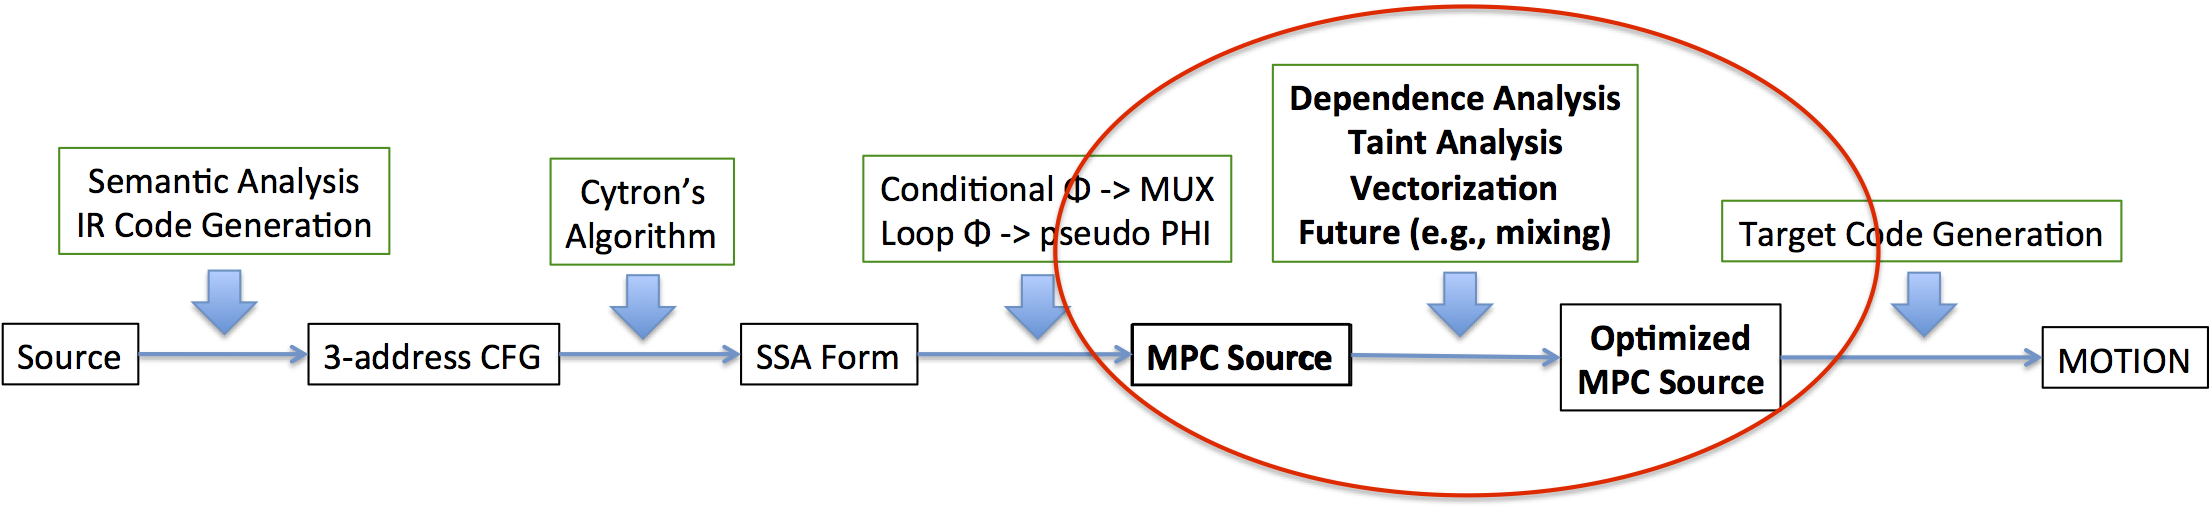
\includegraphics[width=1.0\linewidth]{figs_paper_SIMD/compiler_framework.png}
  \caption{Compiler Framework.} 
  \label{fig:compiler_framework}
\end{figure*}


%We assume arbitrarily nested loops in the MPC-source IR and read-only arrays. We assume that loops range from 0 to some constant N. Arrays are linearized (row-major order as in MOTION) and accesses are via functions of the induction variables of the enclosing loops. 

\figref{fig:compiler_framework} presents an overview of our compiler. In this section, we describe several of the phases of the compiler. 
Sections~\secref{sec:vectorization} and~\secref{sec:div_and_conq} describe vectorization and divide-and-conquer.
We write $i,j,k$ to denote the loop nest: $i$ is the outermost loop, $j$, is immediately nested in $i$, and so on until $k$
and we use $I,J,K$ to denote the corresponding upper bounds. For simplicity, we write $A[i,j,k]$ to denote canonical access 
to an array element. In the program, canonical access is achieved via the standard row-major order formula: $(J*K)*i + K*j + k$.
To simplify the presentation we describe our algorithms in terms of three-element tuples $i,j,k$.
All discussion generalizes to arbitrarily large loop nests.
%\ana{Need to state this more precisely.}

\subsection{Semantic Analysis}

Our compiler performs the following semantic analysis steps:

\begin{enumerate}
  \item
        \textbf{Parsing}:
        Use Python's \texttt{ast} module to parse the input source code to a Python AST.
  \item
        \textbf{Syntax checking}:
        Ensure that the AST matches a restricted subset that our compiler supports.
        This step outputs an instance of the \texttt{restricted\_ast.Function} class, which represents our restricted subset of the Python AST.
  \item
        \textbf{3-address CFG conversion}:
        TODO: Is this a good amount of detail?

        Convert the restricted-syntax AST to a three-address control-flow graph.
        To do this, first,
        add an empty basic block to the CFG and mark it as current.
        Next, for each statement in the restricted AST's function body,
        process the statement.
        Statements can either be for-loops, if-statements, or assignments.
        Rules for processing each kind of statement are given below:
        \begin{enumerate}
          \item
                \textbf{For-loops}:
                Create new basic blocks for
                the loop condition
                (the condition block),
                the loop body
                (the body block),
                and the code after the loop
                (the after-block).
                Insert a jump from the end of the current block to the condition block.
                Then, mark the condition block as the current block.
                Insert a for-instruction at the end of the current block with the loop counter variable and bounds from the AST.
                Next, add an edge from the current block to the after-block labeled ``FALSE'' and
                an edge from the current block to the
                body block labeled ``TRUE''.
                Then, set the body block to be the current block
                and process all statements in the AST's loop body.
                Finally, insert a jump to the condition block and set the after-block as current.
          \item
                \textbf{If-statements}:
                Create new basic blocks for
                the ``then'' statements of the if-statement
                (the then-block),
                the ``else'' statements of the if-statement
                (the else-block),
                and the code after the if-statement
                (the after-block).
                At the end of the current block,
                insert a conditional jump to the then-block or else-block
                depending on the if-statement condition in the AST.
                Next,
                mark the then-block as current,
                process all then-statements,
                and add a jump to the after-block.
                Similarly,
                mark the else-block as current,
                process all else-statements,
                and add a jump to the after-block.
                Finally, set the after-block to be the current block,
                and give it a ``merge condition'' property equal to the condition of the if-statement.
          \item
                \textbf{Assignments}:
                In the restricted-syntax AST,
                the left-hand side of assignments
                can be a variable or an array subscript.
                If it is an array subscript such as \texttt{A[i] = x},
                change the statement to \texttt{A = Update(A, i, x)}.
                If the statement is not already three-address code,
                for each sub-expression in the right-hand side of the assignment,
                insert an assignment to a temporary variable.
        \end{enumerate}
  \item
        \textbf{SSA conversion}:
        Convert the 3-address CFG to SSA with Cytron's algorithm.
\end{enumerate}

\subsection{MUX Nodes and Pseudo $\phi$-nodes}

\ana{Benjamin?}

\ana{I think we need to add more here. Conversion from SSA to MPC Source is not so trivial.}

A pseudo $\phi$-node $X_1 = \phi(X_0,X_2)$ in a loop header is evaluated during circuit generation. If it is the 0-th iteration, then the $\phi$-node evaluates to $X_0$, otherwise, it evaluates to $X_2$.

%\ana{We need to double check that the following captures all cases of def-use edges.}

\subsection{Dependence Analysis}


\subsubsection{Def-use Edges}

The dependence graph has the following def-use edges:

\begin{itemize}
\item same-level edge $X\rightarrow Y$ where $X$ and $Y$ are in the same loop nest, say $i,j,k$. E.g., the def-use edge from \texttt{d = S[i,j] - C[j]} to \texttt{p = d*d} in the Biometric MPC-source is a same-level edge. A same-level edge can be a back-edge in which case a $\phi$ node is the target of the edge. E.g., $\texttt{min}_1 = \mathit{MUX}(\texttt{c},\texttt{sum}_1,\texttt{min}_1)$ to $\texttt{min}_0 = \phi(\texttt{min}_1, 10000)$ in Biometric is a same-level back-edge.
\item outer-to-inner $X\rightarrow Y$ where $X$ is in an outer loop nest, say $i$, and $Y$ is in an inner one, say $i,j,k$. 
%A $\phi$-node can be a source or a target of an outer-to-inner forward edge.
\item inner-to-outer $X\rightarrow Y$ where $X$ is a $phi$-node in an inner loop nest, $i,j,k$, and $Y$ is in the enclosing loop nest $i,j$. E.g. $\texttt{sum}_0 = \phi(\texttt{sum}_1, 0)$ to $\texttt{c} = \mathit{CMP}(\texttt{sum}_0,\texttt{min}_0)$ is an inner-to-outer edge. An inner-to-outer edge can be a back-edge as well in which case both $X$ and $Y$ are phi-nodes with the source $X$ in a loop nested into $Y$'s loop (not necessarily immediately).

%Note that the source is \emph{always} a $\phi$-node of the $i,j,k$ loop and the target is in the immediately enclosing loop. The interpretation of this edge is that the use node $Y$ uses the definition made in the last iteration of the inner loop.
%\ben{The current representation of pseudo $\phi$-nodes shows them attached to the loop header (i.e. in the loop).  We may want to clarify that they are also evaluated at the loop's termination.}
%\item same-level back-edge $X\rightarrow Y$. $Y$ is a phi-node in the header of the loop and $X$ is a definition of the variable in the loop body. E.g., $\texttt{min}_1 = \mathit{MUX}(\texttt{c},\texttt{sum}_1,\texttt{min}_1)$ to $\texttt{min}_0 = \phi(\texttt{min}_1, 10000)$ in Biometric is a same-level back-edge.
%\item inner-to-outer back-edge $X\rightarrow Y$: $X$ and $Y$ are both $\phi$-nodes for some variable. The source $X$ is in a loop nested into $Y$'s loop (not necessarily immediately).

\item mixed forward edge $X\rightarrow Y$. $X$ is in some loop $i,j,k$ and $Y$ is in a loop nested into $i,j,k'$. We transform mixed forward edges as follows. Let $\x$ be the variable defined at $X$. We add a variable and assignment $\x' = \x$ immediately after the $i,j,k$ loop. Then we replace the use of $\x$ at $Y$ with $\x'$. This transforms a mixed forward edge into an "inner-to-outer" forward edge followed by an outer-to-inner forward edge. Thus, Basic Vectorization handles one of "same-level", "inner-to-outer", or "outer-to-inner" def-use edges.
 \end{itemize}

\subsubsection{Closures}

We define $\mathit{closure}(n)$ where $n$ is a phi-node. Intuitively, it computes the set of nodes (i.e., statements) that form a dependence cycle with $n$. The closure of $n$ is defined as follows:
\begin{itemize}
\item $n$ is in $\mathit{closure}(n)$
\item $X$ is in $\mathit{closure}(n)$ if there is a same-level path from $n$ to $X$, and $X \rightarrow n$ is a same-level back-edge.
\item $Y$ is in $\mathit{closure}(n)$ if there is a same-level path from $n$ to $Y$ and there is a same-level path from $Y$ to some $X$ in $\mathit{closure}(n)$.
\end{itemize}

\subsection{Taint Analysis}

We require that all inputs are marked as either shared or plaintext.  We then determine if intermediate variables are shared through taint analysis with "taintedness" referring to the shared attribute.  Specifically, our compiler follows the following rules:
\begin{itemize}
\item If any variable on the right-hand side of an assignment is shared, then the assigned variable is shared
\item If all variables on the right-hand side of an assignment are plaintext, then the assigned variable is plaintext
\item Loop counters are always plaintext
\item Any variables which cannot be determined as shared or plaintext via the above rules are plaintext
\end{itemize}

The first two rules are standard for taint analysis, and the third rule follows from the MPC problem statement. \ben{Is the explanation for the third rule correct?}  The final rule is needed to handle cycles of plaintext values.  For example, in the below snippet \texttt{sum!2} and \texttt{sum!3} form a dependency cycle and cannot be marked as plaintext through simple taint analysis:
{\small
\begin{verbatim}
plaintext_array = [0, 1, 2, ...]
sum!1 = 0
for i in range(0, N):
    sum!2 = PHI(sum!1, sum!3)
    sum!3 = sum!2 + plaintext_array[i]
\end{verbatim}
}
\ben{I think the above example is unnecessary and could be replaced by an explanation of how "untainted" variables are implicitly plaintext, but I couldn't think of a way to phrase that.}

When converting to MOTION code, any plaintext value used in the right-hand side of a shared assignment is implicitly converted to a shared value for that expression. \ben{Is this necessary to include?}

\section{Vectorization}
\label{sec:vectorization}

An important component of our algorithm is the "lifting" of scalars to the corresponding loop dimensionality. 
For example, \texttt{d = S[i * D + j] - C[j]} equiv. to \texttt{d = S[i,j] - C[j]}, which gave rise to \texttt{N*D} subtraction operations in the sequential schedule, 
is lifted. The argument arrays \texttt{S} and \texttt{C} are lifted and the scaler \texttt{d} is lifted: \texttt{d[i,j] = S[i,j] - C[i,j]}.
The algorithm then detects that the statement can be vectorized. 

There are three kinds of arrays (for now all kept internally as one-dimensional arrays, but that's under discussion).
\begin{itemize}

\item Scalars: These are scalar variables we lift into arrays for the purposes of vectorization. 
For those, all writes are canonical writes and all reads are canonical reads. We will apply raise dimension when 
a scalar is used in an inner loop (e.g., \texttt{sum0} in line 6 of the MPC source code will be raised to a 1-dimensional 
array since \texttt{sum0} is used in the inner $j$-loop). Drop dimension applies as well; this happens when a scalar
written in an inner loop is used outside of the loop (e.g., \texttt{sum0} for which the lifted inner loop computes 
\texttt{D} values, but the outer loop only needs the last one.)

\item Read-only input arrays: Read-only inputs. There are NO writes, while we may have non-canonical reads, $f(i,j,k)$. 
Phase 1 of Basic vectorization will add raise dimension operation at the beginning of the function to lift these arrays, 
and raise dimension may \emph{reshape} arrays. If there are multiple "views" of the input array, there would be multiple raise dimension statements to create
each one of these views. The invariant is that at reads in loops, the reads of "views" of the original input array are canonical.
Only raise dimension applies to these arrays, and only in the beginning of the program. For example, 1-dimensional array 
\texttt{C} is lifted into 2-dimensional array \texttt{N x D} by copying the row \texttt{N} times. 
 
 \item Read-write output arrays: Writes are canonical (by restriction) but reads can be non-canonical. 
 Dependence analysis limits vectorization when non-canonical read access refers to array writes in
 previous iterations, thus creating loop-carried dependences. We may apply both raise and drop dimension, however, 
 they respect the fixed dimensionality of the output array. The array cannot be raised to a dimension lower than
 its canonical (fixed) dimensionality and it cannot be dropped lower. In addition, non-canonical reads may 
 require lifting (i.e., reshaping) of the array after the most recent write, rather than in the beginning of the program, 
 in order to reduce a non-canonical read to a canonical one. 

\end{itemize}

In the sections below we detail the $\mathit{raise\_dim}$ (raise dimension) and $\mathit{drop\_dim}$ (drop dimension) operations,
followed by our vectorization algorithm.

%\ana{Add back-edges into Phase 1. A back-edge from a non-phi-node in loop $i$ to a phi-node in loop $i$'s header is a same-level edge. The only difference with the handling of normal same-level forward def-use is that the operand index will become $i-1$. A back edge from a phi-node in loop $j$ to a phi-node in loop $i$, where $j$ is nested in $i$ is an inner-to-outer edge and will require dropping dimension. We can show these are the only kinds of back-edges that may occur.}

%\subsection{Algorithm (Still work in progress.)}

\subsection{Raise Dimension and Drop Dimension}

There are two conceptual versions of $\mathit{raise\_dim}$. One applies on read-only input arrays and reshapes those arrays 
when necessary to ensure canonical read access in the corresponding loop. The signature of $\mathit{raise\_dim}$
is as follows. It takes the original array \texttt{C}, the access pattern function $f(i,j,k)$ in loop nest $i,j,k$ and the loop bounds
\texttt{((i:I),(j:J),(k:K))}: 
\[ \mathit{raise\_dim}(\texttt{A}, f(i,j,k), \texttt{((i:I),(j:J),(k:K))}) \]
It produces a new 3-dimensional array \texttt{A'} by iterating over $i,j,k$ and setting each element of  \texttt{A'} as follows:
\[ \texttt{A'[i,j,k] =  A[f(i,j,k)]} \]
The end result is that uses of \texttt{[A[f(i,jk)]} in loop nest $i,j,k$ are replaced with canonical read-accesses to \texttt{A'[i,j,k]}
that can be vectorized. In the running Biometric example, \texttt{C'} = $\mathit{raise\_dim}$\texttt{(C, j, (i:N,j:D))} lifts the 
1-dimensional array \texttt{C} into a 2-dimensional array. The $i,j$ loop now accesses \texttt{C'} in the canonical way, \texttt{C'[i,j]}. 
Similarly, \texttt{S'} = $\mathit{raise\_dim}$\texttt{(S, i*D+j, (i:N,j:D))} tries to lift \texttt{S}, but the operation turns into a no-op 
because \texttt{S} is already a 2-dimensional array and the read access is canonical. 

The other version of $\mathit{raise\_dim}$ applies on scalars and read-write arrays. It lifts a lower-dimension array into a 
higher-dimension for access in a nested loop. Here \texttt{A} is an $i$ array and raise dimension adds two additional dimensions:
\[ \mathit{raise\_dim}(\texttt{A}, \texttt{(j:J,k:K)}) \]
This version is reduced to the above version by adding the access pattern function, which is just $i$: 
\[ \mathit{raise\_dim}(\texttt{A}, i, \texttt{(j:J,k:K)}) \]

The corresponding $\mathit{drop\_dim}$ is carried out when an array written in an inner loop is used in an enclosing loop. 
It takes a higher dimensional array, say $i,j,k$ and removes trailing dimensions, say $j,k$:
\[ \mathit{drop\_dim}(\texttt{A}, \texttt{(j:J,k:K)}) \]
It iterates over $i$ and takes the result at the maximal index of $j$ and $k$, i.e., the result at the last iterations of $j$ and $k$:
\[ \texttt{A'[i] = A[i,J-1,K-1]} \]


\begin{comment}
We define the $\mathit{raise\_dim}$ (raise dimensions) and $\mathit{drop\_dim}$ (drop dimension) functions. Raise dimension "lifts" a lower-dimension array (\ana{The right term here is tensor, I am pretty sure!}) into a higher dimension one. This is necessary when a lower-dimensional array is used in a higher dimensional loop and, essentially, is just copying of values. For example, Biometric contains the statement $d = \mathit{SUB}(S[i, j], C[j])$, in the $j$-loop which is nested into the $i$-loop. Here $C$ is a one-dimensional array, however, to vectorize across both loops it is necessary to turn it into a two-dimensional array: $C[i,j]$ becomes $[C[0],C[1],...C[J],C[0],C[1],...C[J], ... C[0],C[1],...C[J]]$, which turns the row into a matrix of $I$ identical rows. (We use capital letters to denote the upper bounds of loops, e.g., $J$ is the upper bound of the $j$-loop and $I$ is the upper bound of the $i$-loop.)

$\mathit{raise\_dim}(A[i_1,...,i_k],i_j)$ is defined as follows.  It results in a new {k+1}-dimensional array $A'$ where for every $0 \le i_{k} < I_{k+1}$, $A'[i_1, \ldots, i_j, \ldots, i_k] = A[i_1, \ldots, i_k]$. Adding $n$ dimensions is trivially extended as a composition of $n$ $\mathit{raise\_dim}$ that each adds a single dimension.

As expected, drop dimension turns a higher-dimensional array into a lower-dimensional one. The key use case is an inner-to-outer def-use edge. The code may define a variable, e.g., $\x$ in an inner loop, say $j$, then use this variable in an enclosing loop, say $i$. Our algorithm may vectorize the computation of $\x$ in the $j$-loop thus producing a vector $\x[j]$ where $\x[1]$ is the value of \x after the 1st iteration and so on. Drop dimension states that the outer loop will use the value of the variable at the last iteration.

$\mathit{drop\_dim}(A[i_1,\ldots, i_j, \ldots,i_k], i_j)$ produces a k-dimensional array $A'$ where $A'[i_1,\ldots,i_k] = A'[i_1,\ldots, I_j-1, \ldots,i_k]$. In our analysis, dimensions are always dropped at the end, and again, one can define dropping $n$ dimensions as a composition of $n$ $\mathit{drop\_dim}$.

\ben{I'm not sure if I wrote up the above paragraphs correctly -- the idea is that we're just copying values to extend over dimension $j$ or only retain its last elements.  The current writeup implies that $1 < j < k$ though, which isn't always true.  Python implementations of $\mathit{raise\_dim}()$ and $\mathit{drop\_dim}()$ can be found here: \url{https://github.com/milana2/ParallelizationForMPC/blob/master/compiler/compiler/motion_backend/reference_implementations.py}}

\ana{This section is still informal. Needs work to make more precise.}
\end{comment}

\subsection{Basic Vectorization}

\begin{algorithmic}

\STATE \COMMENT { Phase 1: Raise dimension of scalar variables to corresponding loop nest. We can traverse stmts linearly in MPC-source. }

\FOR {each MPC $\mathit{stmt}: X = \mathit{Op}(Y_1,Y_2)$ in loop $i,j,k$}
%\FOR {each $Y_n$}
\FOR {each argument $Y_n$} %def-use edge $\mathit{stmt}' (\mbox{def of } Y) \rightarrow \mathit{stmt} (\mbox{def of } X)$}
\STATE {case def-use edge $\mathit{stmt}' (\mbox{def of } Y_n) \rightarrow \mathit{stmt} (\mbox{def of } X)$ of} \\
\STATE \hspace{0.25cm} {same-level: $Y'_n$ is $Y_n$} \\
\STATE \hspace{0.25cm} {outer-to-inner: add $Y'_n[i,j,k] = \mathit{raise\_dim}(Y_n)$ at $\mathit{stmt'}$}
\STATE \hspace{0.25cm} {(more precisely, right after $\mathit{stmt'}$)}
\STATE \hspace{0.25cm} {inner-to-outer: add $Y'_n[i,j,k] = \mathit{drop\_dim}(Y_n)$ at $\mathit{stmt}$}
\STATE \hspace{0.25cm} {(more precisely, in loop of $\mathit{stmt}$ right after loop of $\mathit{stmt'}$)}
\ENDFOR

\COMMENT { Optimistically vectorize all. $I$ means vectorized dimension. }
%\FOR {each MPC $\mathit{stmt}: X = \mathit{Op}(Y_1,Y_2)$ in loop $i,j,k$}
\STATE {change to $X[I,J,K] = \mathit{Op}(Y'_1[I,J,K],Y'_2[I,J,K])$ }
\ENDFOR

\COMMENT { Phase 2: Recreating FOR loops for cycles; vectorizable statements hoisted up. }

\FOR {each dimension $d$ from highest to 0}
\FOR {each $\phi$-node $n$ in loop $i_1,...,i_d$}
\STATE {compute $\mathit{closure}(n)$}
\ENDFOR

\COMMENT {{\color{red} $cl_1$ and $cl_2$ intersect if they have common statement or update same array; "intersect" definition can be expanded}}

\WHILE {there are closure $cl_1$ and $cl_2$ that intersect}
\STATE {merge $cl_1$ and $cl_2$}
\ENDWHILE
\FOR {each closure $cl$ (after merge)}
\STATE {create FOR $i_d = 0; ...$ loop}
\STATE {add $\phi$-nodes in $cl$ to header block}
\STATE {{\color{red}{add target-less $\phi$-node for A if $cl$ updates array A}}}
\STATE {add statements in $cl$ to loop body in some order of dependences}
\STATE \COMMENT { Dimension is not vectorizable: }
\STATE {change ${I_d}$ to $i_d$ in all statements in loop}
\STATE {treat FOR loop as monolith node: some def-use edges become same-level.}
\ENDFOR
{
\color{red}
\FOR {each target-less $\phi$-node $A_1 = \phi(A_0,A_k)$}
\STATE {in vectorizable stmts, replace use of $A_1$ with $A_0$}
\STATE {discard $\phi$-node if not used in any $cl$, replacing $A_1$ with $A_0$ or $A_k$ appropriately}
\ENDFOR
}
\ENDFOR

\COMMENT { Phase 3: Remove unnecessary dimensionality. }

\COMMENT { A dimension $i$ is dead on exit from stmt $X[...i...] = ...$ if all def-uses with targets outside of the enclosing 
FOR $i=0 ...$ MOTION loop end at target (use) $X' = \mathit{drop\_dim}(X, i)$. } 
\FOR {each stmt and dimension $X[...i...] = ...$}
\STATE {if $i$ is a dead dimension on exit from stmt $X[...i...] = ...$, remove $i$ from $X$ (all defs and uses)} 
%\COMMENT{ A stmt v[...i] is a "dead dimension i" if all edges out of FOR i = 0; ... loop end at drop\_dim(v, i)}
\ENDFOR

\COMMENT { Now clean up drop\_dim and raise\_dim }
\FOR {each $X' =  \mathit{drop\_dim(X,i)}$ }
\STATE {replace with $X' = X$ if $i$ is dead in $X$.}
\ENDFOR
\STATE {do (1) (extended) constant propagation, (2) copy propagation and (3) dead code elimination to get rid of redundant variables and raise and drop dimension statements}

\COMMENT { Phase 4: }
\STATE {add SIMD for simdified dimensions}

\end{algorithmic}

%\documentclass{article}

%\begin{document}

\subsection{Example: biometric}

\subsubsection{Benjamin's code with linear loops (MPC Source)}

{\small
\begin{verbatim}
min_sum!1 = 10000
min_index!1 = 0
for i in range(0, N!0):
   min_sum!2 = PHI(min_sum!1, min_sum!4)
   min_index!2 = PHI(min_index!1, min_index!4)
   sum!2 = 0
   for j in range(0, D!0):
     sum!3 = PHI(sum!2, sum!4)
     d!3 = (S!0[((i * D!0) + j)] - C!0[j])
     p!3 = (d!3 * d!3)
     sum!4 = (sum!3 + p!3)
   !1!2 = (sum!3 < min_sum!2)
   min_sum!3 = sum!3
   min_index!3 = i
   min_sum!4 = MUX(!1!2, min_sum!3, min_sum!2)
   min_index!4 = MUX(!1!2, min_index!3, min_index!2)
\end{verbatim}
}

\subsubsection{Phase 1 of Basic Vectorization}

The transformation preserves the dependence edges. It raises the dimensions of scalars and optimistically vectorizes all operations. 
The next phase discovers loop-carried dependences and removes affected vectorization.

In the code below, all initializations (e.g., \texttt{min\_sum!3 = i}), operations, and PHI nodes are \emph{implicitly vectorized}. 
$\mathit{raise\_dim}$ and $\mathit{drop\_dim}$ statements, as well as propagation statements (e.g., \texttt{min\_sum!3 = sum!3\^}) 
may have slightly different interpretation. \ana{This is vague, may need elaboration.}

Note the two different versions of $\mathit{raise\_dim}$. \ana{More here! One just adds a least-significant dimension. The other one may reshape an input array.}

{\small
\begin{verbatim}
min_sum!1 = 10000
min_sum!1^ = raise_dim(min_sum!1, (i:N!0))
min_index!1 = 0
min_index!1^ = raise_dim(min_index!1, (i:N!0))
S!0^ = raise_dim(S!0, ((i * D!0) + j), (i:N!0,j:D!0))
C!0^ = raise_dim(C!0, j, (i:N!0,j:D!0))
for i in range(0, N!0):
   min_sum!2 = PHI(min_sum!1^, min_sum!4)
   min_index!2 = PHI(min_index!1^, min_index!4) 
   sum!2 = 0 // Will lift, when hoisted
   sum!2^ = raise_dim(sum!2, (j:D!0)) // Special form?
   for j in range(0, D!0):
      sum!3 = PHI(sum!2^, sum!4)
      d!3 = S!0^ - C!0^
      p!3 = (d!3 * d!3) 
      sum!4 = (sum!3 + p!3)
   sum!3^ = drop_dim(sum!3)     
   !1!2 = (sum!3^ < min_sum!2)
   min_sum!3 = sum!3^
   min_index!3 = i  // Same-level, will lift when hoisted
   min_sum!4 = MUX(!1!2, min_sum!3, min_sum!2)
   min_index!4 = MUX(!1!2, min_index!3, min_index!2)
\end{verbatim}
}

\subsubsection{Phase 2 of Basic Vectorization}

This phase analyzes statements from the innermost loop to the outermost. The key point is to discover loop-carried dependencies and re-introduce loops whenever dependencies make this necessary.

Starting at the inner phi-node \texttt{sum!3 = PHI(sum!2\^, sum!4)}, the algorithm first computes its closure. The closure amounts to the phi-node itself and the addition node \texttt{sum!4 = (sum!3 + p!3)}, accounting for the loop-carried dependency of the computation of \texttt{sum}. The algorithm replaces this closure with a FOR loop on $j$ removing vectoriaztion on $j$. Note that the SUB and MUL computations remain outside of the loop as they do not depend on phi-nodes that are part of cycles. The dependences are from \texttt{p!3[I,J] = (d!3[I,J] * d!3[I,J])} to the monolithic FOR loop and from the FOR loop to \texttt{sum!3\^ = drop\_dim(sum!3)}. (Lower case index, e.g., \texttt{i}, indicates non-vectorized dimension, while uppercase index, e.g., \texttt{I} indicates vectorized dimension.)

After processing inner loop code becomes:

{\small
\begin{verbatim}
min_sum!1 = 10000
min_sum!1^ = raise_dim(min_sum!1, (i:N!0))
min_index!1 = 0
min_index!1^ = raise_dim(min_index!1, (i:N!0))
S!0^ = raise_dim(S!0, ((i * D!0) + j), (i:N!0,j:D!0))
C!0^ = raise_dim(C!0, j, (i:N!0,j:D!0))
for i in range(0, N!0):
  min_sum!2[I] = PHI(min_sum!1^[I], min_sum!4[I]) 
  min_index!2[I] = PHI(min_index!1^[I], min_index!4[I])  
  sum!2 = [0,..,0] 
  sum!2^ = raise_dim(sum!2, (j:D!0))
  d!3[I,J] = S!0^[I,J] - C!0^[I,J]
  p!3[I,J] = (d!3[I,J] * d!3[I,J])
  for j in range(0, D!0):
    sum!3[I,j] = PHI(sum!2^[I,j], sum!4[I,j-1])       
    sum!4[I,j] = (sum!3[I,j] + p!3[I,j])
  sum!3^ = drop_dim(sum!3)     
  !1!2[I] = (sum!3^[I] < min_sum!2[I])
  min_sum!3 = sum!3^
  min_index!3 = [0,1,2,...,N!0-1]
  min_sum!4[I] = MUX(!1!2[I], min_sum!3[I], min_sum!2[I])
   min_index!4[I] = MUX(!1!2[I], min_index!3[I], min_index!2[I])
\end{verbatim}
}

When processing the outer loop two closures arise, one for \texttt{min\_sum!2[I] = PHI(...)} and one 
for \texttt{min\_index!2[I] = PHI(...)}. Since the two closures \emph{do not} intersect, we have two distinct FOR-loops on $i$:

{\small
\begin{verbatim}
min_sum!1 = 10000
min_sum!1^ = raise_dim(min_sum!1, (i:N!0))
min_index!1 = 0
min_index!1^ = raise_dim(min_index!1, (i:N!0))
S!0^ = raise_dim(S!0, ((i * D!0) + j), (i:N!0,j:D!0))
C!0^ = raise_dim(C!0, j, (i:N!0,j:D!0))

sum!2 = [0,..,0]
sum!2^ = raise_dim(sum!2, (j:D!0))
d!3[I,J] = S!0^[I,J] - C!0^[I,J]
p!3[I,J] = (d!3[I,J] * d!3[I,J])

for j in range(0, D!0):
  sum!3[I,j] = PHI(sum!2^[I,j], sum!4[I,j-1])       
  sum!4[I,j] = (sum!3[I,j] + p!3[I,j])

sum!3^ = drop_dim(sum!3)     
min_index!3 = [0,1,2,...N!0-1]   
min_sum!3 = sum!3^

for i in range(0, N!0):
  min_sum!2[i] = PHI(min_sum!1^[i], min_sum!4[i-1]) 
  !1!2[i] = (sum!3^[i] < min_sum!2[i])
  min_sum!4[i] = MUX(!1!2[i], min_sum!3[i], min_sum!2[i])
    
for i in range(0, N!0):
  min_index!2[i] = PHI(min_index!1^[i], min_index!4[i-1])  
   min_index!4[i] = MUX(!1!2[i], min_index!3[i], min_index!2[i])
\end{verbatim}
}

\subsubsection{Phase 3 of Basic Vectorization}

And this phase adds SIMD operations:

{\small
\begin{verbatim}
min_sum!1 = 10000
min_sum!1^ = raise_dim(min_sum!1, (i:N!0))
min_index!1 = 0
min_index!1^ = raise_dim(min_index!1, (i:N!0))
S!0^ = raise_dim(S!0, ((i * D!0) + j), (i:N!0,j:D!0))
C!0^ = raise_dim(C!0, j, (i:N!0,j:D!0))

sum!2 = [0,..,0]
sum!2^ = raise_dim(sum!2, (j:D!0))
d!3[I,J] = SUB_SIMD(S!0^[I,J],C!0^[I,J])
p!3[I,J] = MUL_SIMD(d!3[I,J] * d!3[I,J])

for j in range(0, D!0):
  sum!3[I,j] = PHI(sum!2^[I,j], sum!4[I,j-1])       
  sum!4[I,j] = ADD_SIMD(sum!3[I,j],p!3[I,j])

sum!3^ = drop_dim(sum!3)     
min_index!3 = [0,1,...N!0-1]   
min_sum!3 = sum!3^

for i in range(0, N!0):
  min_sum!2[i] = PHI(min_sum!1^[i], min_sum!4[i-1]) 
  !1!2[i] = CMP(sum!3^[i],min_sum!2[i])
  min_sum!4[i] = MUX(!1!2[i], min_sum!3[i], min_sum!2[i])
    
for i in range(0, N!0):
  min_index!2[i] = PHI(min_index!1^[i], min_index!4[i-1])  
   min_index!4[i] = MUX(!1!2[i], min_index!3[i], min_index!2[i])
\end{verbatim}
}

\ana{TODO: It will be good to add a pass in Phase 3 to get rid of extra dimensionality. 
Once we have vectorized as much as possible, there is no need to keep higher 
dimensionality. E.g., there is no need for the 2-dimensional array sum in the first for loop, 
and similarly, there is no need for 1-dimensional arrays for min\_sum and min\_index.
We should get rid of these before generating MOTION code.}

\ana{Begin Work-in-progress notes on implementation. Just some thoughts...} 

For now, I suggest we go with a "naive" implementation and try to do only minimal optimizations. 
All arrays are stored in the program as one-dimensional arrays. Arrays lifted from scalars have dimensionality of the loop enclosure in 
the original code, e.g., \texttt{sum!3} is two dimensional \texttt{[N!0,D!0]} (but represented linearly in row-major order; all these "copies" are 
arrays of references to shares). Naturally, all writes into these arrays are canonical writes, i.e., $A[i,j] = ...$ and no things like $A[i+1,j-1] = ...$.

The loop "for j in range..." is perhaps the most interesting. First, consider "projection", e.g., p!3[I,j]. 
We fix j (the current iteration) and iterate over I using the row-major formula; it returns the j-th column, 
a one-dimensional column vector. I think this can be generalized across any mix of vectorized vs. 
non-vectorized dimensions but I'm not 100\% sure.

\begin{verbatim}
// project the (j-1)-st column vector:
A = sum!4[I,j-1]
// project j-th column from p!3: 
B = p!3[I,j] 
// we get a N!0-size vector of references to NEW shares:
C = ADD_SIMD(A,B) 
// Writes j-th column of sum!4 with the new references:
sum!4[I,j] = C 
// may eventually optimize since C is A
\end{verbatim}

There are three kinds of arrays (for now all kept internally as one-dimensional arrays, but that's under discussion).
\begin{itemize}

\item Scalars: These are scalar variables we lift into arrays for the purposes of vectorization. 
For those, all writes are canonical writes and all reads are canonical reads. We may apply both raise dimension 
and drop dimension on these.

\item Read-only input arrays: Read-only inputs. There are NO writes, while we may have non-canonical reads, $f(i,j,k)$. 
Phase 1 of Basic vectorization will add raise dimension operation at the beginning of the function and raise dimension 
may reshape arrays. If there are multiple "views" of the input array, there could be multiple raise dimension statements to create
each one of these views. The invariant is that at reads in loops, the reads of "views" of the original input array will be canonical.
Only raise dimension applies.
 
 \item Read-write output arrays: Writes are canonical (by restriction) but reads can be non-canonical. Conjecture:
 do nothing. Dependence analysis takes care of limiting vectorization so non-canonical access will work. 
Still work in progress. We may apply both raise and drop dimension. 

\end{itemize}

\ana{End Work-in-progress notes.}

%\end{document}


\begin{comment}
\subsection{Example: Biometric}

\subsubsection{MPC-source}

Below is the MPC-source resulting from Benjamin's analysis. It gives rise to a corresponding dependence graph. (Not shown.)

\begin{algorithmic}

\STATE \COMMENT {Begin of outer loop $i$.}
\STATE {$\texttt{index}_0 = \phi(-1, \texttt{index}_1)$}
\STATE {$\texttt{min}_0 = \phi(10000,\texttt{min}_1)$}

\STATE \COMMENT {Begin of inner loop $j$.}
\STATE {$\texttt{sum}_0 = \phi(0, \texttt{sum}_1)$}
\STATE {$\texttt{d} = \mathit{SUB}(\texttt{S}[i,j], \texttt{C}[j])$}
\STATE {$\texttt{p} = \mathit{MUL}(\texttt{d},\texttt{d})$}
\STATE {$\texttt{sum}_1 = \texttt{ADD}(\texttt{sum}_0,\texttt{p})$}
\STATE \COMMENT {End of inner loop $j$.}
\STATE {$\texttt{c} = \mathit{CMP}(\texttt{sum}_0,\texttt{min}_0)$}
\STATE {$\texttt{index}_1 = \mathit{MUX}(\texttt{c},\texttt{index}_0,i)$}
\STATE {$\texttt{min}_1 = \mathit{MUX}(\texttt{c},\texttt{min}_0,\texttt{sum}_0)$}
\STATE \COMMENT {End of outer loop $i$.}

\end{algorithmic}

\subsubsection{Phase 1 of Basic Vectorization:}

The transformation preserves the dependence edges. It raises the dimensions of scalars and optimistically vectorizes all operations. The next phase discovers loop-carried dependences and removes affected vectorization.

\begin{algorithmic}

\STATE \COMMENT {Begin of outer loop $i$.}
\STATE {$\texttt{index}_0[i] = \phi(-1,\texttt{index}_1[i-1])$}
\STATE {$\texttt{min}_0[i] = \phi(10000, \texttt{min}_1[i-1])$}

\STATE \COMMENT {Begin of inner loop $j$.}
\STATE {$\texttt{sum}_0[i,j] = \phi([0,0,...], \texttt{sum}_1[i,j-1])$}
\STATE {$\texttt{C}'[i,j] = \mathit{raise\_dim}(\texttt{C}[j],i)$}
\STATE {$\texttt{d}[\stackrel{\rightarrow}{i},\stackrel{\rightarrow}{j}] = \mathit{SUB}(\texttt{S}[\stackrel{\rightarrow}{i},\stackrel{\rightarrow}{j}], \texttt{C}'[\stackrel{\rightarrow}{i},\stackrel{\rightarrow}{j}])$}
\STATE {$\texttt{p}[\stackrel{\rightarrow}{i},\stackrel{\rightarrow}{j}] = \mathit{MUL}(\texttt{d}[\stackrel{\rightarrow}{i},\stackrel{\rightarrow}{j}],\texttt{d}[\stackrel{\rightarrow}{i},\stackrel{\rightarrow}{j}])$}
\STATE {$\texttt{sum}_1[\stackrel{\rightarrow}{i},\stackrel{\rightarrow}{j}] = \mathit{ADD}(\texttt{sum}_0[\stackrel{\rightarrow}{i},\stackrel{\rightarrow}{j}],\texttt{p}[\stackrel{\rightarrow}{i},\stackrel{\rightarrow}{j}])$}
\STATE \COMMENT {End of inner loop $j$.}
\STATE {$\texttt{sum}'_0[i] = \mathit{drop\_dim}(\texttt{sum}_0[i,j],j)$}
\STATE {$\texttt{c}[\stackrel{\rightarrow}{i}] = \mathit{CMP}(\texttt{sum}'_0[\stackrel{\rightarrow}{i}],\texttt{min}_0[\stackrel{\rightarrow}{i}])$}
\STATE {$\texttt{index}_1[\stackrel{\rightarrow}{i}] = \mathit{MUX}(\texttt{c}[\stackrel{\rightarrow}{i}],\texttt{index}_0[\stackrel{\rightarrow}{i}],[0,1,...N])$}
\STATE {$\texttt{min}_1[\stackrel{\rightarrow}{i}] = \mathit{MUX}(\texttt{c}[\stackrel{\rightarrow}{i}],\texttt{min}_0[\stackrel{\rightarrow}{i}],\texttt{sum}'_0[\stackrel{\rightarrow}{i}])$}
\STATE \COMMENT {End of outer loop $i$.}

\end{algorithmic}

\ishaq{At least for input variables: when raising dimensions, we should keep some meta data around so we can later write code that could use 1 share if it knows the other N shares are just duplicates of it.}

\subsubsection{Phase 2}

This phase analyzes statements from the innermost loop to the outermost. The key point is to discover loop-carried dependencies and re-introduce loops whenever dependencies make this necessary.

Starting at the inner phi-node $\texttt{sum}_0[i,j] = \phi([0,0,...],\texttt{sum}_1[i,j-1])$, the algorithm first computes its closure. The closure amounts to the phi-node itself and $\texttt{sum}_1[\stackrel{\rightarrow}{i},\stackrel{\rightarrow}{j}] = \mathit{ADD}(\texttt{sum}_0[\stackrel{\rightarrow}{i},\stackrel{\rightarrow}{j}],\texttt{p}[\stackrel{\rightarrow}{i},\stackrel{\rightarrow}{j}])$, accounting for the loop-carried dependency of the computation of \texttt{sum}. The algorithm replaces this closure with a FOR loop on $j$ removing vectoriaztion on $j$. Note that the SUB and MUL computations remain outside of the loop as they do not depend on phi-nodes that are part of cycles. The algorithm adds same-level edges, one from $\texttt{p}[\stackrel{\rightarrow}{i},\stackrel{\rightarrow}{j}] = ...$ to the monolithic FOR-loop node, and one from the FOR-loop node to $\texttt{c}[\stackrel{\rightarrow}{i}] = ...$.

\ishaq{For our radar: Such dependencies will not involve phi nodes only. e.g. $a[i] = a[i] + a[i-1]$}

\begin{algorithmic}

\STATE \COMMENT {Begin of outer loop $i$.}
\STATE {$\texttt{index}_0[i] = \phi(-1, \texttt{index}_1[i-1])$}
\STATE {$\texttt{min}_0[i] = \phi(10000, \texttt{min}_1[i-1])$}



\STATE {$\texttt{C}'[i,j] = \mathit{raise\_dim}(\texttt{C}[j],i)$}
\STATE {$\texttt{d}[\stackrel{\rightarrow}{i},\stackrel{\rightarrow}{j}] = \mathit{SUB}(\texttt{S}[\stackrel{\rightarrow}{i},\stackrel{\rightarrow}{j}], \texttt{C}'[\stackrel{\rightarrow}{i},\stackrel{\rightarrow}{j}])$}
\STATE {$\texttt{p}[\stackrel{\rightarrow}{i},\stackrel{\rightarrow}{j}] = \mathit{MUL}(\texttt{d}[\stackrel{\rightarrow}{i},\stackrel{\rightarrow}{j}],\texttt{d}[\stackrel{\rightarrow}{i},\stackrel{\rightarrow}{j}])$}

\STATE \COMMENT {Begin of inner loop $j$. Loop is now much "shorter"!}
\STATE {$\texttt{sum}_0[i,j] = \phi([0,0,...], \texttt{sum}_1[i,j-1])$}
\STATE {FOR j=0; j<D; j++} \COMMENT{ Will turn into a MOTION loop.}
\STATE \hspace{0.25cm}{$\texttt{sum}_1[\stackrel{\rightarrow}{i},{j}] = \mathit{ADD}(\texttt{sum}_0[\stackrel{\rightarrow}{i},{j}],\texttt{p}[\stackrel{\rightarrow}{i},{j}])$}
\STATE \COMMENT {End of inner loop $j$.}

\STATE {$\texttt{sum}'_0[i] = \mathit{drop\_dim}(\texttt{sum}_0[i,j],j)$}
\STATE {$\texttt{c}[\stackrel{\rightarrow}{i}] = \mathit{CMP}(\texttt{sum}'_0[\stackrel{\rightarrow}{i}],\texttt{min}_0[\stackrel{\rightarrow}{i}])$}
\STATE {$\texttt{index}_1[\stackrel{\rightarrow}{i}] = \mathit{MUX}(\texttt{c}[\stackrel{\rightarrow}{i}],\texttt{index}_0[\stackrel{\rightarrow}{i}],[0,1,...N])$}
\STATE {$\texttt{min}_1[\stackrel{\rightarrow}{i}] = \mathit{MUX}(\texttt{c}[\stackrel{\rightarrow}{i}],\texttt{min}_0[\stackrel{\rightarrow}{i}],\texttt{sum}'_0[\stackrel{\rightarrow}{i}])$}
\STATE \COMMENT {End of outer loop $i$.}

\end{algorithmic}

Next, analysis moves to outer dimension $i$. There are two phi-nodes, $\texttt{min}_0[i] = \phi(10000,\texttt{min}_1[i-1])$ and $\texttt{index}_0[i] = \phi(-1,\texttt{index}_1[i-1])$.
The closure of the first is
\[
\begin{array}{l}
\texttt{min}_0[i] = \phi(10000,\texttt{min}_1[i-1]) \\
\texttt{c}[\stackrel{\rightarrow}{i}] = \mathit{CMP}(\texttt{sum}'_0[\stackrel{\rightarrow}{i}],\texttt{min}_0[\stackrel{\rightarrow}{i}]), \\
\texttt{min}_1[\stackrel{\rightarrow}{i}] = \mathit{MUX}(\texttt{c}[\stackrel{\rightarrow}{i}],\texttt{min}_0[\stackrel{\rightarrow}{i}],\texttt{sum}'_0[\stackrel{\rightarrow}{i}])
\end{array}
\]
and the closure of the second one is
\[
\begin{array}{l}
\texttt{index}_0[i] = \phi(-1,\texttt{index}_1[i-1]), \\
%\texttt{c}[\stackrel{\rightarrow}{i}] = \mathit{CMP}(\texttt{sum}'_1[\stackrel{\rightarrow}{i}],\texttt{min}_0[\stackrel{\rightarrow}{i}]), \\
\texttt{index}_1[\stackrel{\rightarrow}{i}] = \mathit{MUX}(\texttt{c}[\stackrel{\rightarrow}{i}],\texttt{index}_0[\stackrel{\rightarrow}{i}],[0,1,...N])
\end{array}
\]

Since the two closures \emph{do not} intersect, we have two distinct FOR-loops on $i$. The first FOR loop (on \texttt{min}) is scheduled first, because of the dependence edge from $\texttt{c}[\stackrel{\rightarrow}{i}] = \mathit{CMP}(\texttt{sum}'_0[\stackrel{\rightarrow}{i}],\texttt{min}_0[\stackrel{\rightarrow}{i}])$ to
$\texttt{index}_1[\stackrel{\rightarrow}{i}] = \mathit{MUX}(\texttt{c}[\stackrel{\rightarrow}{i}],\texttt{index}_0[\stackrel{\rightarrow}{i}],[0,1,...N])$. We can now rewrite those statements, getting rid of the vectorization on $i$ in the two FOR loops. Notably, the SUB and MUL computations are fully vectorizable and the ADD computation is vectorizable across the $i$-dimension.

\begin{algorithmic}

\STATE
\STATE {$\texttt{C}'[i,j] = \mathit{raise\_dim}(\texttt{C}[j],i)$}
\STATE {$\texttt{d}[\stackrel{\rightarrow}{i},\stackrel{\rightarrow}{j}] = \mathit{SUB\_SIMD}(\texttt{S}[\stackrel{\rightarrow}{i},\stackrel{\rightarrow}{j}], \texttt{C}'[\stackrel{\rightarrow}{i},\stackrel{\rightarrow}{j}])$}
\STATE {$\texttt{p}[\stackrel{\rightarrow}{i},\stackrel{\rightarrow}{j}] = \mathit{MUL\_SIMD}(\texttt{d}[\stackrel{\rightarrow}{i},\stackrel{\rightarrow}{j}],\texttt{d}[\stackrel{\rightarrow}{i},\stackrel{\rightarrow}{j}])$} \\
\STATE {}
\STATE {$\texttt{sum}_0[i,j] = \phi([0,0,...],\texttt{sum}_1[i,j-1])$}
\STATE {FOR j=0; j<D; j++} \COMMENT{ Turns into a MOTION loop, was $j$-loop.}
\STATE \hspace{0.25cm}{$\texttt{sum}_1[\stackrel{\rightarrow}{i},{j}] = \mathit{ADD\_SIMD}(\texttt{sum}_0[\stackrel{\rightarrow}{i},{j}],\texttt{p}[\stackrel{\rightarrow}{i},{j}])$}
\STATE {}
\STATE {$\texttt{sum}'_0[i] = \mathit{drop\_dim}(\texttt{sum}_0[i,j],j)$}
\STATE {}
\STATE {$\texttt{min}_0[i] = \phi(10000,\texttt{min}_1[i-1])$}
\STATE {FOR i=0; i<N; i++} \COMMENT{ Turns into a MOTION loop, was $i$-loop.}
\STATE \hspace{0.25cm}{$\texttt{c}[{i}] = \mathit{CMP}(\texttt{sum}'_0[{i}],\texttt{min}_0[{i}])$}
\STATE \hspace{0.25cm}{$\texttt{min}_1[{i}] = \mathit{MUX}(\texttt{c}[{i}],\texttt{min}_0[{i}],\texttt{sum}'_1[{i}])$}
\STATE {}
\STATE {$\texttt{index}_0[i] = \phi(-1,\texttt{index}_1[i-1])$}
\STATE {FOR i=0; i<N; i++} \COMMENT{ Turns into a MOTION loop, was $i$-loop.}
\STATE \hspace{0.25cm}{$\texttt{index}_1[{i}] = \mathit{MUX}(\texttt{c}[{i}],\texttt{index}_0[{i}],i)$}

\ben{The above code implicitly stores the final values of min\_0 and index\_0 in their last indices, but there is no primitive like drop\_dim to make it clear.  This will have to be added in the SSA code generation (though it might not be necessary to include in the paper?).  It also is pretty wishy-washy about the size and layout of each vector (again more of an implementation issue), but maybe we should have a different syntax for array accesses for read/write (e.g. the ADD\_SIMD steps) vs the array definitions (e.g. the SUB\_SIMD and raise/drop\_dim statements)}

\end{algorithmic}
\end{comment}

\subsection{Correctness Argument}

We build a correctness argument that loosely follows the theory of Abstract Interpretation. 
We define the syntax of MPC Source programs. The domain of MPC Source programs
expressible in the syntax (with certain semantic restrictions) is the abstract domain $A$. 
We then define the \emph{linearization} of an MPC Source program as an interpretation 
over the syntax. The linearization, which is a \emph{schedule}, is the concrete domain $C$. 
Since we reason over def-use graphs in $A$ we define a partial order relation over elements of $A$ 
in terms of def-use relations. We define a partial order over elements of $C$ as well,
in terms of def-use relations in the concrete domain $C$. We prove two theorems
that state (informally) that the schedule corresponding to the original program computes the same 
result as the schedule corresponding to the vectorized program.


\begin{figure}%[!b]
%\small
\[
\begin{array}{l@{~~~~~}l}
  \begin{array}{l@{~}l@{~~~}l}
  s &::= s;s & sequence \\
     & \mid \x[i,J,k] = \y[i,J,k] \; \mathit{op\_SIMD} \; \z[i,J,k] & operation \\ 
     & \mid \x[i,J,k]  = \texttt{PHI}(\x_1[i,J,k],\x_2[i,J,k\!-\!1]) & \mathit{phi} \; \mathit{node} \\
     & \mid \x[i,J,k] = \mathit{raise\_dim}(\x'[i],(J\!:\!J,k\!:\!K)) & \mathit{raise} \; \mathit{dimension(s)} \\
     & \mid \x[i,J] = \mathit{drop\_dim}(\x'[i,J,k],k)  & \mathit{drop} \; \mathit{dimension(s)} \\
     & \mid \x = \y & \mathit{propagation} \\
     & \mid \texttt{FOR} \; 0 \le i < I: s  & \mathit{loop} \\
  \end{array}    \\
\end{array}
\]
\vspace{-3mm}
\caption{MPC Source Syntax}\label{fig:MPC_Source_syntax}
\vspace{-5mm}
\end{figure}

\paragraph{MPC Source Syntax}

\figref{fig:MPC_Source_syntax} defines the syntax for our intermediate representation, MPC Source. 
There are semantics restrictions over the syntax as well: a variable $\x[i,j,k]$ is a 3-dimensional array 
$(i:I,j:J,k:K)$ and also, a statement $\x[i,J,k] = ...$ is enclosed in loops over $i$ and $k$ as shown below. 
Thus, $i$ and $k$ are in scope.
\begin{verbatim}
FOR 0 <= i < I:
    ...
    FOR 0 <= k < K:
        x[i,J,k] = ...
\end{verbatim}

Statements $\mathit{operation, phi, raise \; dimension(s), drop \; dimension(s)}$ are \emph{base} statements, 
and $\mathit{sequence, loop}$ are \emph{compound statements}.

\paragraph{Linearization}

Linearization is the concretization operation, which, as we mentioned earlier computes a schedule.
The concretization function $\gamma: A \rightarrow C$ is defined as an interpretation of
MPC Source syntax, as it is standard. The concretization of each one 
of the base statements is as follows: 
\[\begin{array}{l}
\gamma(\x[i,J,k] = \mathit{op\_SIMD}(\y[i,J,k], \z[i,J,k])) = \\ 
~~\x[i,0,k] = \y[i,0,k] \; \mathit{op} \; \z[i,0,k] \;\; || \\
~~~~\x[i,1,k] = \y[i,1,k] \; \mathit{op} \; \z[i,1,k] \;\; || \; ...\; || \\
~~~~~~\x[i,I-1,k] = \y[i,I-1,k] \; \mathit{op} \; \z[i,I-1,k]
\end{array}\]
meaning that the vectorized dimension(s) are expanded into parallel statements. || introduces SIMD (parallel) execution.

The concretization of the FOR statement is as follows:
\[ \gamma(\texttt{FOR} \; 0 \le i < I: s) = \gamma(s)[0/i] \; ; \; \gamma(s)[1/i] \; ; \; ... \gamma(s)[I-1/i] \]
$\gamma$ simply unrolls the loop substituting $i$ with 0, 1, etc. Here ; denotes sequential execution.

\paragraph{Partial Orders}

For each MPC Source program $a$ we compute the def-use edges in the standard way: if base statement $s1 \in a$ defines variable \x, e.g., $\x[i,j,k] = ...$, 
and base statement $s2 \in a$ uses \x, e.g., $... = ... \x[i,j,k]$ and there is a path in the trivial CFG from $s1$ to $s2$, then there is a def-use edge from
 $s1$ to $s2$. We extend the dimensionality of a statement into $s1[i,j,k]$ where $s1[i,j,k]$ inherits the dimensionality of the left-hand-side of the assignment.
  
 Let $a_0, a_1$ be two MPC Source programs in $A$. 
 Two base statements, $s_0 \in a_0$ and $s_1 \in a_1$ are \emph{same}, written $s_0 \equiv s_1$ if they are of the same operation and they operate on 
 the same variables: same variable name and same dimensionality. Recall that dimensions in MPC Source are either iterative, lower case, or vectorized, upper case. 
 Two statements are same even if one operates on an iterative dimension and the other one operates on a vectorized one, e.g., $s_0[i,j,k] \equiv s_1[I,j,K]$.
  
 \begin{definition} Let $a_0, a_1 \in A$. We say that $a_0 \le a_1$ iff for every def-use edge $s1 \rightarrow s2$ in $a_0$ there is an edge
 $s1' \rightarrow s2'$ where $s1 \equiv s1'$, $s2 \equiv s2'$ and the two edges of either both forward or both backward.
 \end{definition}
 
 The def-use edges in the concrete schedule are as expected. There is a def use edge from statement $s1$ that defines $\x[\underline{i},\underline{j},\underline{k}]$
 to statement $s2$ that uses $\x[\underline{i},\underline{j},\underline{k}]$ if $s1$ is scheduled ahead of $s2$ in the linear schedule. We note that the underlined
 indices, e.g., $\underline{i}$, refer to fixed values, not iterative or vectorized dimensions since in the concrete schedule all induction variables are expanded. 
 E.g., there is a def-use edge from the statement that defines $\x[0,1,2]$ and a statement that uses $\x[0,1,2]$.
 
\paragraph{Theorems} 

\begin{theorem} $a_0 \le a_1 \Rightarrow \gamma(a_0) \subseteq \gamma(a_1)$.
\end{theorem}

\begin{theorem} Let $a_0$ be the iterative MPC Source and let $a_1$ be the vectorized MPC Source computed by the vectorization algorithm. 
We have that $a_0 \le a_1$. 
\end{theorem}

\ana{Write the proof sketch and final argument, etc.}

\subsection{Extension of Basic Vectorization with Array Writes}

\subsubsection{Removal of Infeasible Edges}

Array writes limit vectorization as they sometimes introduce infeasible loop-carried dependencies. Consider the following example: \ana{Have to add citation to Aiken's paper}

{\small
\begin{verbatim}
for i in range(N):
  A[i] = B[i] + 10;
  B[i] = A[i] * D[i-1];
  C[i] = A[i] * D[i-1];
  D[i] = B[i] * C[i];
\end{verbatim}
}

In Cytron's SSA this code (roughly) translates into

{\small
\begin{verbatim}
for i in range(N):
1. A_1 = PHI(A_0,A_2)
2. B_1 = PHI(B_0,B_2)
3. C_1 = PHI(C_0,C_2)
4. D_1 = PHI(D_0,D_2)
5. A_2 = update(A_1, i, B_1[i] + 10); 
6. B_2 = update(B_1, i, A_2[i] * D_1[i-1]);
7. C_2 = update(C_1, i, A_2[i] * D_1[i-1]);
8. D_2 = update(D_1, i, B_2[i] * C_2[i]);
\end{verbatim}
}

\begin{comment}
\begin{algorithmic}
\STATE for i in range(N):
\STATE \hspace{0.25cm} A[i] = B[i] + 10;
\STATE \hspace{0.25cm} B[i] = A[i] * D[i-1];
\STATE \hspace{0.25cm} C[i] = A[i] * D[i-1];
\STATE \hspace{0.25cm} D[i] = B[i] * C[i];
\end{algorithmic}

\begin{algorithmic}
\STATE for i in range(N):
\STATE 1. $\texttt{A}_0$ = $\phi(\texttt{A},\texttt{A}_1)$
\STATE 2. $\texttt{B}_0$ = $\phi(\texttt{B},\texttt{B}_1)$
\STATE 3. $\texttt{C}_0$ = $\phi(\texttt{C},\texttt{C}_1)$
\STATE 4. $\texttt{D}_0$ = $\phi(\texttt{D},\texttt{D}_1)$
\STATE 5. $\texttt{A}_1$ = $\texttt{A}_0$; $\texttt{A}_1$[i] = $\texttt{B}_0$[i] + 10; \COMMENT{equiv. to Update}
\STATE 6. $\texttt{B}_1$ = $\texttt{B}_0$; $\texttt{B}_1$[i] = $\texttt{A}_1$[i] * $\texttt{D}_0$[i-1];
\STATE 7. $\texttt{C}_1$ = $\texttt{C}_0$; $\texttt{C}_1$[i] = $\texttt{A}_1$[i] * $\texttt{D}_0$[i-1];
\STATE 8. $\texttt{D}_1$ = $\texttt{D}_0$; $\texttt{D}_1$[i] = $\texttt{B}_1$[i] * $\texttt{C}_1$[i];
\end{algorithmic}
\end{comment}

There is a cycle around \texttt{B\_1 = PHI(B\_0,B\_2)} that includes statement 
\texttt{A\_1 = update(A\_0, i, B\_1[i] + 10)} and that statement won't be vectorized even 
though in fact there is no loop-carried dependency from the write of \texttt{B\_1[i]} at 6 to the
read of \texttt{ ... = B\_1[i]} at 8.

The following algorithm removes certain infeasible loop-carried dependencies that are due to array writes. Consider a loop with index $0 \le j < J$
nested at $i,j,k$. Here $i$ represents the enclosing loops of $j$ and $k$ represents the enclosed loops in $j$.

\begin{algorithmic}
\FOR {each array $\texttt{A}$ written in loop $j$}
\STATE \COMMENT { including enclosed loops in $j$ }
\STATE dep = False
\FOR {each pair def: $\texttt{A}_m[f(i,j,k)] = ... $, and use: $ ... = \texttt{A}_n[f'(i,j,k)]$ in loop $j$}
\IF {$\exists \underline{i}, \underline{j}, \underline{j}', \underline{k}, \underline{k}'$, s.t. $0\! \le\! \underline{i}\! <\! I,\: 0\! \le\! \underline{j}, \underline{j}' \! <\! J,\: 0\! \le\! \underline{k}, \underline{k}' \! <\! K,\: \underline{j}<\underline{j}'$, and $f(\underline{i},\underline{j},\underline{k}) = f'(\underline{i},\underline{j}',\underline{k}')$}
\STATE dep = True
\ENDIF
\ENDFOR
\IF {dep == False}
\STATE remove back edge into $\texttt{A}$'s $\phi$-node in loop $j$.
\ENDIF
\ENDFOR
\end{algorithmic}

Consider a loop $j$ enclosed in some fixed $\underline{i}$. Only if an update (definition) $\texttt{A}_m[f(i,j,k)] = ... $ at some iteration $\underline{j}$
references the \emph{same} array element as a use $ ... = \texttt{A}_n[f'(i,j,k)]$ at some later iteration $\underline{j}'$,
we may have a loop-carried dependence for $\texttt{A}$ due to this def-use pair. (In contrast, Cytron's algorithm inserts a loop-carried dependency every time there is an array update.)
The algorithm above examines all def-use pairs in loop $j$, including defs and uses in nested loops, searching for values $\underline{i}, \underline{j}, \underline{j}', \underline{k}, \underline{k}'$ that satisfy
$f(\underline{i},\underline{j},\underline{k}) = f'(\underline{i},\underline{j}',\underline{k}')$. If such values exist for some def-use pair, then there is a potential
loop-carried dependence on $\texttt{A}$; otherwise there is not and we can remove the spurious backward edge thus ``freeing up'' statements for vectorization. %\ana{Double check this!!!}

Consider the earlier example. There is a single loop, $i$. Clearly, there is no pair $\underline{i}$ and $\underline{i}'$, where $\underline{i} < \underline{i}'$ that make $\underline{i} = \underline{i}'$ 
due to the def-use pairs of \texttt{A} 5-6 and 5-7.
Therefore, we remove the back edge from 5 to the phi-node 1. Analogously, we remove the back edges from 6 to 2 and from 7 to 3. However, there are many values $\underline{i} < \underline{i'}$ that make $\underline{i} = \underline{i'}-1$ and the back edge from 8 to 4 remains (def-use pairs for \texttt{D}). As a result of removing these spurious edges, Basic Vectorization will find that statement 5 is vectorizable. Statements 6, 7 and 8 will correctly appear in the FOR loop.

Note however, that this step renders some array phi-nodes target-less. We handle target-less phi-nodes with a minor extension of Basic Vectorization (Phase 2). 
First, we merge closures that update the same array. This simplifies handling of array $\phi$-nodes: if each closure is turned into a separate loop
each loop will need to have its own array phi-node to account for the update and this would complicate the analysis.
Second, we add the target-less node of array \texttt{A} back to the closure that updates \texttt{A} ---
the intuition is, even if there is no loop-carried dependence from writes to reads on \texttt{A}, \texttt{A} is written and the write (i.e., update) cannot be vectorized; 
therefore, the updated array has to carry to the next iteration of the loop. Third, in cases when the phi-node remains target-less, i.e., cases when the
array write can be vectorized, we have to properly remove the phi-node replacing uses of the left-hand side of the phi-node with its arguments.

%\ana{Commented out previous writeup. Removal/handling of targetless phi-nodes will go into the Extension to Basic vectorization.}

\begin{comment}
The final step is to remove array phi-nodes that are left without incoming back edges after removal of infeasible edges.
Such a phi-node is redundant when there are no loop-carried dependences that are due to writes to the corresponding array.
In our running example, the phi-nodes for \texttt{A}, \texttt{B}, and \texttt{C}, are redundant.

Removing redundant phi-nodes proceeds from \emph{innermost to outermost} loops as follows.
Denote a redundant phi-node by $\texttt{A}_1 = \phi(\texttt{A}_0,\texttt{A}_k)$. $\texttt{A}_0$ is the array at the beginning of the loop
and $\texttt{A}_k$ is the array at the end of an iteration (including the last iteration). We consider two cases:
\begin{enumerate}
\item[Case 1] Inner-to-outer or same-level def-use edge
\begin{itemize}
\item If use is an array read $ ... = \texttt{A}_1[f(i)]$, then replace $\texttt{A}_1$ with $\texttt{A}_0$. This is correct, i.e., it is guaranteed that the use
references $\texttt{A}_0$; had the use been referencing an array modified in an earlier iteration, the back-edge to the phi-node would
not have been removed and the phi-node would not have been classified as redundant.
\item If use is an array write (update) $\texttt{A}_2 = \texttt{A}_1; \texttt{A}_2[i] = ... $ equiv. to $\texttt{A}_2 = \mathit{update}(\texttt{A}_1, i, ...)$ then handling becomes more tricky.
The semantics of this update is that when $i$ is 0, then $\texttt{A}_0$ is being read. But when $i > 0$, then $\texttt{A}_k$ is being read. If we are at this case, this means that the def-use edge is same-level and we are removing a redundant node in the loop enclosing the update. The removal of the original phi-node entails pushing the phi-node at the update:
$\texttt{A}_2 = \phi(\texttt{A}_0,\texttt{A}_k); \texttt{A}_2[i] = ... $ equiv. to $\texttt{A}_2 = \mathit{update}(\phi(\texttt{A}_0,\texttt{A}_k), i, ...)$.
\item If use is a phi-node $... = \phi(\texttt{A}_1,...)$, that means we have an outer-to-inner edge. The

\end{itemize}
\end{enumerate}
For each outer-to-inner or same-level def-use edge
that originates at the node, replace $\texttt{A}_1$ at the use node by $\texttt{A}_0$.
For each inner-to-outer def-use edge, replace $\texttt{A}_1$ by $\texttt{A}_k$. In this case, the use references the array
that results from the computation in the loop.

Our running example is transformed as follows. Removing the phi-nodes for \texttt{A}, \texttt{B}, and \texttt{C} transforms the
replaces the references to $\texttt{A}_0$, $\texttt{B}_0$, and $\texttt{C}_0$, with references to $\texttt{A}$, $\texttt{B}$, and $\texttt{C}$
respectively, i.e., the arrays before the loop.

\begin{algorithmic}
\STATE for i in range(N):
\STATE 1. $\texttt{D}_0$ = $\phi(\texttt{D},\texttt{D}_1)$
\STATE 2. $\texttt{A}_1$ = $\texttt{A}$; $\texttt{A}_1$[i] = $\texttt{B}$[i] + 10;
\STATE 3. $\texttt{B}_1$ = $\texttt{B}$; $\texttt{B}_1$[i] = $\texttt{A}_1$[i] * $\texttt{D}_0$[i-1];
\STATE 4. $\texttt{C}_1$ = $\texttt{C}$; $\texttt{C}_1$[i] = $\texttt{A}_1$[i] * $\texttt{D}_0$[i-1];
\STATE 5. $\texttt{D}_1$ = $\texttt{D}_0$; $\texttt{D}_1$[i] = $\texttt{B}_1$[i] * $\texttt{C}_1$[i];
\end{algorithmic}
\end{comment}

\subsubsection{Array MUX refinement}

\ana{TODO: WIP, get to BV without MUX refinement for now? For now, skip MUX refinement.}

Next, the algorithm refines array MUX statements.
MPC-source after Cytron's SSA may result in statements $\texttt{A}_j = \emph{MUX}(..., \texttt{A}_k, \texttt{A}_l)$, which imply that any index
of A can be written at this point and therefore there is a loop-carried dependency. In some cases the MUX can be refined to just a single
index or a pair of indices, e.g., $\texttt{A}_j[i] = \emph{MUX}(c, \texttt{A}_k[i], \texttt{A}_l[i])$.

%\ana{Clarify why this helps. Still work in progress.}
This is to reduce the dimensionality of simd-ified computation. Technically, $\texttt{A}_j = \emph{MUX}(..., \texttt{A}_k, \texttt{A}_l)$ is
a simdified operation that can be carried out in parallel "in one round". However, particularly when \texttt{A} is a multi-dimensional array, there is
substantial increase in the size of the arrays (vectors) we send to SIMD operations. Refining to an update to a specific index would reduce
the size of those vectors. Note that this is a heuristic that handles a common case, but not all cases of array updates.
%\ana{TODO: Simplify this algorithm, taking into account the restriction to canonical updates. It should be handling \_all\_ cases.}


\begin{algorithmic}
\FOR {each $\mathit{stmt}$: $\texttt{A}_j = \emph{MUX}(c, \texttt{A}_k, \texttt{A}_l)$ in the MPC-source seq.}
\STATE $i_1 = \mathit{find\_update}(A_k)$ \COMMENT { Is null when $A_k = \phi(...)$ }
\STATE $i_2 = \mathit{find\_update}(A_l)$ \COMMENT { Is null when $A_l = \phi(...)$ }
\IF {$i_1 == i_2$ or $i_1$ is null or $i_2$ is null} \STATE \COMMENT{ With our restrictions on writes we must have $i_1 = i_2$. }
\STATE replace $\mathit{stmt}$ with \\
\STATE $\texttt{A}_j = \texttt{A}_{j-1}$; $\texttt{A}_j[i_1] = \emph{MUX}(c, \texttt{A}_k[i_1], \texttt{A}_l[i_1])$
%\ELSIF {$i_1 \ncong i_2$}
%\STATE replace $\mathit{stmt}$ with \\
%\STATE $\texttt{A}_j = \texttt{A}_k$; $\texttt{A}_j[i_1] = \emph{MUX}(c, \texttt{A}_k[i_1], \texttt{A}_l[i_1])$
\ELSE
\STATE $\mathit{stmt}$ stays as is
\ENDIF
\ENDFOR
\end{algorithmic}


\subsubsection{Restricting Array Writes}

For now, we restrict array updates to \emph{canonical updates}. Assume (for simplicity) a two-dimensional array \texttt{A[I,J]}. A canonical update is the following:
\begin{verbatim}
for i in range(I):
  for j in range(J):
    ...
    A[i,j] = ...
    ...
\end{verbatim}

The update \texttt{A[i,j]} can be nested into an inner loop and there may be multiple updates, i.e., writes to \texttt{A[i,j]}. However, update such as \texttt{A[i-1,j] = ...} or \texttt{A[i-1,j-1] = ...}, etc., is not allowed. Additionally, while there could be several different loops that perform canonical updates, they must be of the same dimensionality, i.e., an update of higher or lower dimension, e.g., \texttt{A[i,j,k] = ...} is not allowed. We compute the \emph{canonical dimensionality} of each write array by examining the array writes in the original program and rejecting programs that violate the canonical write restriction. This restriction simplifies reasoning in this early stage of the compiler; we will look to relax the restriction in future work.

Another restriction/assumption is that we assume the output array is given as input with initial values, and it is of size consistent with its canonical dimensionality. 
%\ana{This restriction will require that we update our benchmarks that come with output arrays.}

Reads through an arbitrary formula, such as \texttt{A[i-1]} for example, are allowed; currently, the projection function returns dummy values if the read formula is out of bounds; we assume the programmer ensures that the program still computes correct output in this case.

\subsubsection{Changes to Basic Vectorization}

\begin{comment}
There are two changes to Basic Vectorization to account for write arrays. We can account for them during processing of raise dimension/drop dimension in Phase 1 of Basic Vectorization.

One change to Basic vectorization is the expansion of dimension if the array write or read occurs in a nested loop. That is, if there is an update $\texttt{A}[i,j] = ...$ that occurs in loop dimensionality $i,j,k$, $\texttt{A}[i,j]$ will be rewritten into $\texttt{A}[i,j,k]$. Similarly, a read $\texttt{A}[f(i,j)]$ will be rewritten into $\texttt{A}[f(i,j),k]$. ($\texttt{A}[f(i,j),k]$ will be reshaped as $f(i,j)*I*J+k$ during Phase 1 of Basic Vectorization. \ana{TODO: Double check.}) 
\end{comment}

In addition to the changes for the handling of target-less phi-nodes, Basic Vectorization has to handle def-use edges $X \rightarrow Y$ where $X$ defines and $Y$ uses an array variable. The definition can be an update \texttt{A\_2 = update(A\_1,i,...)}, a pseudo $\phi$-node \texttt{A\_2 = PHI(A\_0,A\_1)}, etc.. Note that $\phi$-nodes for arrays have no subscript operations the way there are subscript operations in analysis-introduced arrays representing scalars. While there are variations, the most intuitive implementation will perform Basic Vectorization Phase 1 as is, inserting 
$\mathit{raise\_dim}$ and $\mathit{drop\_dim}$ in the same way. However, the implementation of raise dimension and drop dimension will be adapted because the dimension cannot be raised or dropped to a dimension lower than the canonical one. Consider a def-use edge $X \rightarrow Y$ for an array $\texttt{A}$.

\begin{enumerate}

\item same-level $X \rightarrow Y$. Do nothing, propagate the array, which happens to be of the right dimension. 
%\ana{There might be some opportunities to do copy propagation optimization and save some cycles, but let's leave this for later.}

\item inner-to-outer $X \rightarrow Y$ triggers the addition of $\mathit{drop\_dim}$. However, the dimensionality cannot be dropped below the canonical dimensionality of the array. E.g., if the dimensionality of the loop enclosure $X$ is already at the canonical one, then $\mathit{drop\_dim}$ has no effect.

\item outer-to-inner $X \rightarrow Y$ riggers  $\mathit{raise\_dim}$. Again, if the dimensionality of the loop enclosure of $Y$ is smaller or same as the canonical dimensionality of the array, then it has no effect, otherwise, if dimensionality is greater than the canonical dimensionality, $\mathit{raise\_dim(...)}$ (at $X$) is the same as in Basic Vectorization.

\item "mixed" $X \rightarrow Y$. We assume that the mixed edge is transformed into an inner-to-outer followed by outer-to-inner edge before we perform vectorization, just as with Basic vectorization.

\end{enumerate}

If the use of the array is a read $\texttt{A}[f(i,j,k)]$ different than a canonical read $\texttt{A}[i,j,k]$, then we need to add a reshape operation as 
all arrays are $\texttt{A}[i,j,k]$. It can be added after raise\_dim/drop\_dim or incorporated in these operations.
The bulk of the change is in Phase 2 of Basic Vectorization as outlined earlier.

\subsubsection{Examples with Array Writes}

\paragraph{Example 1}

First, the canonical dimensionality of all \texttt{A,B,C} and \texttt{D} is 1. 
After Phase 1 of Basic Vectorization the Aiken's array write example will be (roughly) as follows:

{\small
\begin{verbatim}
for i in range(N):
1. A_1 = PHI(A_0,A_2)
2. B_1 = PHI(B_0,B_2)
3. C_1 = PHI(C_0,C_2)
4. D_1 = PHI(D_0,D_2)
5. A_2 = update(A_1, I, B_1[I] + 10); 
6. B_2 = update(B_1, I, A_2[I] * D_1[I-1]);
7. C_2 = update(C_1, I, A_2[I] * D_1[I-1]);
8. D_2 = update(D_1, I, B_2[I] * C_2[I]);
\end{verbatim}
}

Note that since all def-uses are same-level (i.e., reads and writes of the array elements) 
no raise dimension or drop dimension happens.

\begin{comment}
\begin{algorithmic}
\STATE for i in range(N):
\STATE 1. $\texttt{A}_1$ = $\phi(\texttt{A}_0,\texttt{A}_2)$
\STATE 2. $\texttt{B}_1$ = $\phi(\texttt{B}_0,\texttt{B}_2)$
\STATE 3. $\texttt{C}_1$ = $\phi(\texttt{C}_0,\texttt{C}_2)$
\STATE 4. $\texttt{D}_1$ = $\phi(\texttt{D}_0,\texttt{D}_2)$
\STATE 5. $\texttt{A}_2 = update(\texttt{A}_1, \stackrel{\rightarrow}{i}, \texttt{B}_1[\stackrel{\rightarrow}{i}] + 10)$;
\STATE 6. $\texttt{B}_2 = update(\texttt{B}_1, \stackrel{\rightarrow}{i}, \texttt{A}_2[\stackrel{\rightarrow}{i}] * \texttt{D}_1[\stackrel{\rightarrow}{i-1}])$;
\STATE 7. $\texttt{C}_2 = update(\texttt{C}_1, \stackrel{\rightarrow}{i}, \texttt{A}_2[\stackrel{\rightarrow}{i}] * \texttt{D}_1[\stackrel{\rightarrow}{i-1}])$;
\STATE 8. $\texttt{D}_2 = update(\texttt{D}_1; \stackrel{\rightarrow}{i}, \texttt{B}_2[\stackrel{\rightarrow}{i}] * \texttt{C}_2[\stackrel{\rightarrow}{i}])$;
\end{algorithmic}
\end{comment}

Phase 2 computes the closure of 4; $cl = \{4,6,7, 8\}$ 
while 5 is vectorizable. Recall that 1,2, and 3 are target-less phi-nodes. Since the closure $cl$ includes updates to \texttt{B} and \texttt{C},
the corresponding phi-nodes are added back to the closure and the def-use edges are added back to the target-less nodes. The uses of \texttt{A\_1} and \texttt{B\_1} in the vectorized statement
turn into uses of \texttt{A\_0} and \texttt{B\_0} respectively; this is done for all original target-less phi-node. (But note that \texttt{A\_0} is irrelevant; the update writes into array \texttt{A\_2} in parallel.)
Finally, the target-less phi-node for \texttt{A} is discarded. 

{\small
\begin{verbatim}
1. A_2 = update(A_0, I, ADD_SIMD(B_0[I],10));
   equiv. to A_2[I] = ADD_SIMD(B_0[I],10)
FOR i=0; i<N; i++; // MOTION loop
2. B_1 = PHI(B_0,B_2)
3. C_1 = PHI(C_0,C_2)
4. D_1 = PHI(D_0,D_2)
5. B_2 = update(B_1, i, A_2[i] * D_1[i-1]);
   equiv. to B_2 = B_1; B_2[i] = A_2[i] * D_1[i-1];
6. C_2 = update(C_1, i, A_2[i] * D_1[i-1]);
7. D_2 = update(D_1, i, B_2[i] * C_2[i]);
\end{verbatim}
}



\begin{comment}
\begin{algorithmic}
\STATE 1. $\texttt{A}_2 = update(\texttt{A}_0; \stackrel{\rightarrow}{i}, \mathit{ADD\_SIMD}(\texttt{B}_0[\stackrel{\rightarrow}i],[10,...])$ \COMMENT{Fully vectorized, size N.}
\STATE FOR i=0; i<N; i++; \COMMENT{ MOTION loop }
\STATE 2. $\texttt{B}_1$ = $\phi(\texttt{B}_0,\texttt{B}_2)$
\STATE 3. $\texttt{C}_1$ = $\phi(\texttt{C}_0,\texttt{C}_2)$
\STATE 4. $\texttt{D}_1$ = $\phi(\texttt{D}_0,\texttt{D}_2)$
\STATE 5. $\texttt{B}_2 = update(\texttt{B}_1, i, \mathit{MUL}(\texttt{A}_2[i], \texttt{D}_1[{i-1}])$
\STATE 6. $\texttt{C}_2 = update(\texttt{C}_1, i, \mathit{MUL}(\texttt{A}_2[i], \texttt{D}_1[{i-1}])$
\STATE 7. $\texttt{D}_2 = update(\texttt{D}_1, i, \mathit{MUL}(\texttt{B}_2[i], \texttt{C}_1[i])$
\end{algorithmic}
\end{comment}

\paragraph{Example 2} Now consider the MPC Source of Histogram:

{\small
\begin{verbatim}
for i in range(0, num_bins):
   res1 = PHI(res, res2)
   for j in range(0, N):
      res2 = PHI(res1, res3)
      tmp1 = (A[j] == i)
      tmp2 = (res2[i] + B[j])
      tmp3 = MUX(tmp1, res2[i], tmp2)
      res3 = Update(res2, i, tmp3)     
return res1
\end{verbatim}
}

The canonical dimensionality of \texttt{res} is 1. Also, the phi-node \texttt{res1 = PHI(res, res2)} is a target-less phi-node (the implication being that the inner for loop can be vectorized across $i$). After Phase 1, Basic vectorization produces the following code (statements are implicitly vectorized along $i$ and $j$). In a vectorized update statement, we can ignore the incoming array, \texttt{res2} in this case. The update writes (in parallel) all locations of the 2-dimensional array, in this case it sets up each \texttt{res3[i,j] = tmp3[i,j]}.

{\small
\begin{verbatim}
A1 = raise_dim(A, j, ((i:num_bins),(j:N)))
B1 = raise_dim(B, j, ((i:num_bins),(j:N)))
I = raise_dim(i, ((i:num_bins),(j:N)))
for i in range(0, num_bins):
   res1 = PHI(res, res2') // target-less phi-node
   res1' = raise_dim(res1, (j:N))
   for j in range(0, N):
      res2 = PHI(res1', res3)
      tmp1 = (A1 == I)
      tmp2 = (res2 + B1)
      tmp3 = MUX(tmp1, res2, tmp2)
      res3 = Update(res2, (I,J), tmp3) 
   res2' = drop_dim(res2)    
res1'' = drop_dim(res1)
return res1''
\end{verbatim}
}

Processing the inner loop in Phase 2 vectorizes \texttt{tmp1 = (A1 == I)} along the $j$ dimension but leaves the rest of the statements in a MOTION loop. Processing the outer loop is interesting. This is because the PHI node is a target-less node, and therefore, there are no closures! Several things happen. (1) Everything can be vectorized along the $i$ dimension. (2) We remove the target-less PHI node, however, we must update uses of \texttt{res1} appropriately: the use at raise\_dim goes to the first argument of the PHI function and the use at drop\_dim goes to the second argument.

{\small
\begin{verbatim}
A1 = raise_dim(A, j, ((i:num_bins),(j:N)))
B1 = raise_dim(B, j, ((i:num_bins),(j:N)))
I1 = raise_dim(i, ((i:num_bins),(j:N)))

tmp1[I,J] = (A1[I,J] == I1[I,J])

res1' = raise_dim(res, (j:N)) // replacing res1 with res, 1st arg
for j in range(0, N):
   res2 = PHI(res1', res3)
   tmp2[I,j] = (res2[I,j] + B1[I,j])
   tmp3[I,j] = MUX(tmp1[I,j], res2[I,j], tmp2[I,j])
   res3 = Update(res2, (I,j), tmp3)
   equiv. to res3 = res2; res3[I,j] = tmp3[I,j]
res2' = drop_dim(res2)   
res1 = drop_dim(res2') // replacing with res2', 2nd arg. NOOP
return res1
\end{verbatim}
}

\begin{comment}
The cleanup phase can then get rid of $j$ in the \texttt{res} variables and \texttt{tmp} variables, so the loop operates over the \texttt{num\_bins}-size vectors. 
This will lead to dropping raise\_dim and drop\_dim as well: 

{\small
\begin{verbatim}
A1 = raise_dim(A, j, ((i:num_bins),(j:N)))
B1 = raise_dim(B, j, ((i:num_bins),(j:N)))
I1 = raise_dim(i, ((i:num_bins),(j:N)))

tmp1[I,J] = (A1[I,J] == I1[I,J])

for j in range(0, N):
   res2 = PHI(res1, res3) // now 1-dim array
   tmp2[I] = ADD_SIMD(res2[I],B1[I,j])
   tmp3[I] = MUX_SIMD(tmp1[I,j], res2[I], tmp2[I])
   res3 = Update(res2, I, tmp3[I])
return res2
\end{verbatim}
}
\end{comment}

\begin{comment}
\paragraph{Example 2}

Consider MPC-source of Histogram after removal of infeasible edges and redundant phi-nodes, and MUX refinement:

\begin{algorithmic}

\STATE res!1 = []
\STATE for i: plaintext in range(0, num\_bins):
\STATE \hspace{0.25cm} res!2 = $\phi$(res!1, res!3)
\STATE  \hspace{0.25cm} ...
\STATE res!4 = res!2 \COMMENT{Added due to the "mixed" def-use edge.}
\STATE for i: plaintext in range(0, num\_bins):
%\STATE \hspace{0.25cm}        result!4 = $\phi$(result!2, result!5)
\STATE \hspace{0.25cm}        for j: plaintext in range(0, N):
\STATE \hspace{0.5cm}            res!5 = $\phi$(res!4, res!7)
\STATE \hspace{0.5cm}            !2!3 = (A[j] == i)
\STATE \hspace{0.5cm}            !3!3 = (res!5[i] + B[j])
\STATE \hspace{0.5cm}            res!6 = res!5; res!6[i] = !3!3
\STATE \hspace{0.5cm}            res!7 = res!6; res!7[i] = MUX(!2!3, res!6[i], res!5[i])

\end{algorithmic}

After Phase 1 of Basic Vectorization:

\begin{algorithmic}
\STATE res!1 = []
\STATE for i: plaintext in range(0, num\_bins):
\STATE \hspace{0.25cm} res!2 = $\phi$(res!1, res!3)
\STATE  \hspace{0.25cm} ...
\STATE res!4 = res!2 \COMMENT{Added due to the "mixed" def-use edge. Because the canonical dimensionality of res is 1, we DO NOT drop dimension of res!2.}
\STATE A[$i,j$] = $\mathit{raise\_dim}$(A[$j$],$i$) \COMMENT{Copying row A num\_bin times. Reusing name.}
\STATE B[$i,j$] = $\mathit{raise\_dim}$(B[$i$],$j$) \COMMENT{Copying column B N times. Reusing name.}
\STATE res!4[$i,j$] = $\mathit{raise\_dim}$(res!4[$i$],$j$) \COMMENT{Reusing name.}
\STATE for i: plaintext in range(0, num\_bins):
%\STATE \hspace{0.25cm}        result!4 = $\phi$(result!2, result!5)
\STATE \hspace{0.25cm}        for j: plaintext in range(0, N):
\STATE \hspace{0.5cm}            res!5 = $\phi$(res!4, res!7) \COMMENT{Do nothing. res!4 has been raised to proper dimension.}
\STATE \hspace{0.5cm}            !2!3[$\stackrel{\rightarrow}i,\stackrel{\rightarrow}j$] = $\mathit{EQ}$(A[$\stackrel{\rightarrow}i,\stackrel{\rightarrow}j$], [[0,0...], [1,1...],...[num\_bins-1,num\_bins-1...]])
\STATE \hspace{0.5cm}            !3!3[$\stackrel{\rightarrow}i,\stackrel{\rightarrow}j$] = $\mathit{ADD}$(res!5[$\stackrel{\rightarrow}i,\stackrel{\rightarrow}j$],B[$\stackrel{\rightarrow}i,\stackrel{\rightarrow}j$])
\STATE \hspace{0.5cm}            res!6 = res!5 \COMMENT{Do nothing, just copy.}
\STATE \hspace{0.5cm}            res!6[$\stackrel{\rightarrow}i,\stackrel{\rightarrow}j$] = !3!3[$\stackrel{\rightarrow}i,\stackrel{\rightarrow}j$]
\STATE \hspace{0.5cm}            res!7 = res!6
\STATE \hspace{0.5cm}            res!7[$\stackrel{\rightarrow}i,\stackrel{\rightarrow}j$] = $\mathit{MUX}$(!2!3[$\stackrel{\rightarrow}i,\stackrel{\rightarrow}j$], res!6[$\stackrel{\rightarrow}i,\stackrel{\rightarrow}j$], res!5[$\stackrel{\rightarrow}i,\stackrel{\rightarrow}j$])
\end{algorithmic}

After Phase 2 and Phase 3. The EQ operation is vectorizable across both dimensions, and the rest of the computation is vectorizable across the $i$-dimension.

\begin{algorithmic}
\STATE ...
\STATE !2!3[$\stackrel{\rightarrow}i,\stackrel{\rightarrow}j$] = $\mathit{EQ\_SIMD}$(A[$\stackrel{\rightarrow}i,\stackrel{\rightarrow}j$], [[0,0...], [1,1...],...[num\_bins-1,num\_bins-1...]])
%\STATE \hspace{0.25cm}        result!4 = $\phi$(result!2, result!5)
\STATE FOR j=0; j<N; j++; \COMMENT{MOTION loop}
\STATE \hspace{0.25cm}            res!5 = $\phi$(res!4, res!7) \COMMENT{Do nothing, just copy.}
\STATE \hspace{0.25cm}            !3!3[$\stackrel{\rightarrow}i,j$] = $\mathit{ADD\_SIMD}$(res!5[$\stackrel{\rightarrow}i,j$],B[$\stackrel{\rightarrow}i,j$])
\STATE \hspace{0.25cm}            res!6 = res!5 \COMMENT{Do nothing, just copy.}
\STATE \hspace{0.25cm}            res!6[$\stackrel{\rightarrow}i,j$] = !3!3[$\stackrel{\rightarrow}i,j$]
\STATE \hspace{0.25cm}            res!7 = res!6
\STATE \hspace{0.25cm}            res!7[$\stackrel{\rightarrow}i,j$] = $\mathit{MUX\_SIMD}$(!2!3[$\stackrel{\rightarrow}i,j$], res!6[$\stackrel{\rightarrow}i,j$], res!5[$\stackrel{\rightarrow}i,j$])
\end{algorithmic}
\end{comment}


\section{Divide-and-Conquer}
\label{sec:div_and_conq}

\ana{TODO: Now that we have broken FOR loops into smaller chunks, we can add Divide-and-conquer reasoning with Z3 and implement this additional transform.}

\section{Implementation and Evaluation}
\label{sec:implementation}


\section{Future Work}
\label{sec:implementation_and_benchmarks}
%\input{../sections/implementation_and_benchmarks.tex}
%\input{../sections/evaluation.tex}

\section{Conclusions}
\label{sec:conclusion}
%\input{../sections/conclusion.tex}

%\begin{acks}
%    \ishaq{TODO}
%\end{acks}

\printbibliography

% that's all folks
\end{document}


